%% LaTeX Beamer presentation template (requires beamer package)
%% see http://latex-beamer.sourceforge.net/
%% idea contributed by H. Turgut Uyar
%% template based on a template by Till Tantau
%% this template is still evolving - it might differ in future releases!

\documentclass[hyperref={pdfpagelabels=false}]{beamer}

\mode<presentation>

% $Id: macros.tex,v 1.4 2013/08/18 16:00:29 ganeshau Exp $
%\usepackage[pdftex]{hyperref}
\frenchspacing
\usepackage{mathptmx}

%\usepackage{cite}
\usepackage[T1]{fontenc}
\usepackage{times}
\usepackage{url}
%\usepackage{cite}
\usepackage{amsmath}
% \usepackage{fancyhdr}
%\usepackage{fancyvrb}
%\usepackage{fancybox}
\usepackage{color}
\usepackage{colortbl}
\usepackage{mathpartir}
\usepackage{amssymb}
\usepackage{xspace}
\usepackage{comment}
\usepackage{graphicx}
\graphicspath{{figures/}}
%\usepackage{epsfig}
%\usepackage{wrapfig}
\usepackage{multirow}
%\usepackage{subfig}

% Added listing for code listings
\usepackage{listings}
\usepackage{relsize}
%\usepackage{stfloats}
\usepackage{fixltx2e}
\usepackage{courier}
% formatting for grammars
% \input{obey}
% \input{grammar}

\usepackage{soul}
\newcommand{\hlc}[2][yellow]{ {\sethlcolor{#1} \hl{#2}} }

%\renewcommand{\nonterm}[1]{\mbox{\textit{#1}}}
\newcommand{\oneormore}[1]{#1\ensuremath{^+}}

% % %\newcommand{\panini}{\textsf{java}$_c$\xspace}
% \newcommand{\mechanism}{active module\xspace}
% \newcommand{\Mechanism}{Active module\xspace}
% \newcommand{\MEchanism}{Active Module\xspace}
% \newcommand{\mechanisms}{active modules\xspace}
% \newcommand{\Mechanisms}{Active modules\xspace}
% \newcommand{\MEchanisms}{Active Modules\xspace}
%\newcommand{\intermechanism}{inter-modular\xspace}
%\newcommand{\intramechanism}{intra-modular\xspace}

\newcommand{\mechanism}{capsule\xspace}
\newcommand{\Mechanism}{Capsule\xspace}
\newcommand{\MEchanism}{Calsupe\xspace}
\newcommand{\mechanisms}{capsules\xspace}
\newcommand{\Mechanisms}{Capsules\xspace}
\newcommand{\MEchanisms}{Capsules\xspace}
\newcommand{\intermechanism}{inter-capsular\xspace}
\newcommand{\intramechanism}{intra-capsular\xspace}

\newcommand{\MRB}{Message Ring Buffer\xspace}
\newcommand{\mrb}{message ring buffer\xspace}
\newcommand{\TaskFramework}{task framework\xspace}

% Type checking macros
% change symbol type of : from mathrel 
%\DeclareMathSymbol{:}{\mathbin}{operators}{"3A} 
\newcommand{\OK}{\mbox{OK}}
\newcommand{\OKin}{\mbox{OK in }}
\newcommand{\inC}{\mbox{in }c}
\newcommand{\isType}{\mbox{\textit{isType}}}
\newcommand{\validFields}{\mbox{\textit{validF}}}
\newcommand{\isClass}{\mbox{\textit{isClass}}}
\newcommand{\isHandler}{\mbox{\textit{isHandler}}}
\newcommand{\Types}{\mbox{\textit{Types}}}
\newcommand{\Names}{\mbox{\textit{Names}}}
\newcommand{\TypeEnv}{\mbox{\textit{TypeEnv}}}
\newcommand*{\findMeth}{\auxFunc{findMeth}}
\newcommand*{\fieldsOf}{\auxFunc{fields}}
\newcommand*{\fieldName}{\auxFunc{fieldName}}
\newcommand*{\checkMethods}{\auxFunc{methE}}
\newcommand*{\methodEffect}{\auxFunc{me}}
\newcommand*{\typeOfField}{\auxFunc{typeOfF}}
\newcommand*{\typeOf}{\auxFunc{typeOf}}
\newcommand*{\dom}{\auxFunc{dom}}
\newcommand*{\rng}{\auxFunc{rng}}
\newcommand*{\isAnn}{\auxFunc{annotated}}
\newcommand*{\updateEffect}{\auxFunc{update}}
\newcommand*{\reversePointer}{\auxFunc{reverse}}
\newcommand*{\reversePoint}{\auxFunc{reverseP}}
\newcommand*{\fixPoint}{\auxFunc{fixPoint}}
\newcommand*{\updateOther}{\auxFunc{updateOther}}
\newcommand*{\updateMethodEffect}{\auxFunc{updateEff}}
\newcommand*{\updateSingleMethodEffect}{\auxFunc{updateMeth}}
\newcommand*{\updateSingleEffect}{\auxFunc{concretize}}
\newcommand*{\updateForkEffect}{\auxFunc{updateFork}}
\newcommand*{\updateQueue}{\auxFunc{updateQ}}
\newcommand*{\getActive}{\auxFunc{active}\xspace}
\newcommand*{\field}{\auxFunc{field}}
\newcommand{\fdecl}{\mbox{\textit{fdecl}}}
\newcommand*{\fieldOf}{\auxFunc{fieldOf}}
\newcommand*{\getOpen}{\auxFunc{getOpen}}
\newcommand{\NPE}{\mbox{\textit{NPE}}}

% Reserved words (in math mode)
\newcommand{\Extends}{\mbox{\texttt{\textbf{extends}}}}
\newcommand{\Implements}{\mbox{\texttt{\textbf{implements}}}}
\newcommand{\This}{\mbox{\texttt{\textbf{this}}}}
\newcommand{\Self}{\mbox{\texttt{\textbf{self}}}}
\newcommand{\EV}{\mbox{\texttt{\textbf{event}}~}}
\newcommand{\Cast}{\mbox{\texttt{\textbf{cast}}}}
\newcommand{\New}{\mbox{\texttt{\textbf{new}}~}}
\newcommand{\Null}{\mbox{\texttt{\textbf{null}}}}
\newcommand{\Chain}{\mbox{\texttt{\textbf{chain}}~}}
\newcommand{\Under}{\mbox{\texttt{\textbf{under}}~}}
\newcommand{\If}{\mbox{\texttt{\textbf{if}}}}
\newcommand{\Then}{\mbox{\texttt{\textbf{then}}}}
\newcommand{\Else}{\mbox{\texttt{\textbf{else}}}}
\newcommand{\While}{\mbox{\texttt{\textbf{while}}}}

% Aux functions
\newcommand{\auxFunc}[1]{\ensuremath{\mathop{\mathit{#1}}}}
\newcommand*{\override}{\auxFunc{override}}

% types
\newcommand{\POWERSET}[1]{\mbox{\textit{PowerSet}}(#1)}
\newcommand{\delete}{\mbox{\textit{delete}}}
\newcommand{\mklist}{\mbox{\textit{mksupers}}}
\newcommand{\uminus}{\mbox{$\cup\!\!\!\!-$}}
\newcommand{\iminus}{\mbox{$\cap\!\!\!\!-$}}
\newcommand{\commutesWith}{\sharp}
\newcommand{\notCommutesWith}{\not\sharp}
\newcommand{\rname}[1]{$\TirName{(#1)}$} % for inline inferrule names
\newcommand{\STO}{\ensuremath{<:}}  % ``subtype of''
\newcommand{\notSTO}{\ensuremath{\not<:}}  % ``subtype of''
\newcommand{\consistent}{\ensuremath{\approx}}

% auxiliary funtions for finding the dynamic effects for program executions.
\newcommand*{\dynamicInfinite}{\auxFunc{dynValue}}
\newcommand*{\dynamicEffects}{\auxFunc{dynE}}
\newcommand*{\dynamicEffectsOnce}{\auxFunc{dyn}}
\newcommand*{\dynamicEffectSet}{\auxFunc{dynESet}}
\newcommand*{\predecessorSiblings}{\auxFunc{preS}}
\newcommand*{\predSibles}{\auxFunc{pSib}}
%\newcommand*{\offspring}{\auxFunc{descendentsOf}}
%\newcommand*{\offspring}{\auxFunc{descendents}}
\newcommand*{\offspring}{\auxFunc{desc}}
\newcommand*{\offspringOrItself}{\auxFunc{descendOrSelf}} 
\newcommand*{\inQueueX}{\auxFunc{inQ}} 
\newcommand*{\inQueueY}{\auxFunc{inq}}
\newcommand*{\replaceQueue}{\auxFunc{replace}}
\newcommand*{\substituteSequence}{\auxFunc{subSeq}}
\newcommand*{\combineSequence}{\auxFunc{comSeq}}
\newcommand*{\mergeSequence}{\auxFunc{merSeq}}
\newcommand*{\isin}{\auxFunc{belongs}}
\newcommand*{\configuration}{c}

% Macros for operational semantics
\newcommand{\mc}[1]{\mbox{\rm \ensuremath{\text{\code{#1}}}}} % Arg set in code font in math
\newcommand{\loc}{\ensuremath{\mathord{\mathit{loc}}}}
\newcommand{\handler}[3]{\ensuremath{\langle#1,#2,#3\rangle}}
\newcommand{\ec}{\ensuremath{\mathbb{E}}}
%\newcommand{\ec}{\ensuremath{\mathop{\mathbb{E}}}}
%\newcommand{\ecpending}{\ensuremath{\mathop{\mathbb{E'}}}}
\newcommand{\ecpending}{\ensuremath{\mathop{\overline{\mathbb{E}}}}}
\newcommand{\hole}{\ensuremath{\mathord{\mathit{-}}}}
\newcommand{\reducesto}{\hookrightarrow}
\newcommand{\reducestostar}{\overset{*}{\reducesto}}
\newcommand{\dontcare}{\ensuremath{\mathord{\text{\textvisiblespace\hspace{0.10ex}}}}}
\newcommand{\Expression}{\ensuremath{{\cal E}}}
\newcommand{\Stack}{\mbox{\textit{Stack}}}
\newcommand{\Store}{\mbox{\textit{Store}}}
\newcommand{\ActiveList}{\mbox{\textit{ActiveList}}}
\newcommand{\Frame}{\mbox{\textit{Frame}}}
\newcommand{\FieldEnv}{\mbox{\textit{FieldEnv}}}
\newcommand{\ObjectRecord}{\mbox{\textit{ObjectRecord}}}
\newcommand{\lexframe}{\mbox{\textbf{\texttt{frame}}}}
\newcommand{\handlerframe}{\mbox{\textbf{\texttt{hframe}}}}
\newcommand{\Excep}{\mbox{\textit{Excep}}}

\newcommand*{\seq}[1]{\ensuremath{\left\langle {#1} \right\rangle}} % Arg is sequence contents
\newcommand{\config}{\seq}
\newcommand{\udot}{\mathbin{\sqcup \kern-0.53em \cdot \,}}

\newcommand{\eseq}{\hat{e}}

% Effect attributes
\newcommand{\ReadE}{\mbox{\texttt{\textbf{read}}~}}
%\newcommand{\WriteE}{\mbox{\texttt{\textbf{write}}~}}
\newcommand{\WriteE}{\mbox{\texttt{\textbf{write}}~}}
\newcommand{\CheckE}{\mbox{\texttt{\textbf{open}}}}
%\newcommand{\ForkE}{\mbox{\texttt{\textbf{fork}}}}
\newcommand{\ForkE}{\mbox{\texttt{\textbf{fork}}}}
\newcommand{\EnqueueE}{\mbox{\texttt{\textbf{bottom}}}}
%\newcommand{\BottomE}{\mbox{\texttt{\textbf{\bot}}}}
\newcommand{\RegisterE}{\mbox{\texttt{\textbf{exp}}}}
%\newcommand{\AnnounceE}{\mbox{\texttt{\textbf{frk}}~}}
\newcommand{\CreateE}{\mbox{\texttt{\textbf{create}}~}}
% Effect Auxiliary Functions
\newcommand*{\EffectsOf}{\auxFunc{effects}}
\newcommand{\ReadF}{\mbox{\texttt{\textbf{rd}}}}
\newcommand{\WriteF}{\mbox{\texttt{\textbf{wt}}}}
\newcommand{\ForkF}{\mbox{\texttt{\textbf{fk}}}}
\newcommand{\EnqueueF}{\mbox{\texttt{\textbf{eq}}}}
\newcommand{\BottomF}{\mbox{\texttt{\textbf{bt}}}}
\newcommand{\ConcretizedF}{\mbox{\texttt{\textbf{ct}}}}
\newcommand{\OtherF}{\mbox{\texttt{\textbf{el}}}}


\newcommand{\Class}{\mbox{\texttt{\textbf{class}}~}}
\newcommand{\tasks}{\mbox{\texttt{\textbf{tasks}}~}}
\newcommand{\fork}{\mbox{\texttt{\textbf{fork}}~}}
\newcommand{\foreach}{\mbox{\texttt{\textbf{forall}}~}}
\newcommand{\Decl}{\mbox{\texttt{\textbf{decl}}~}}
\newcommand{\RDecl}{\mbox{\texttt{\textbf{rdecl}}~}}
\newcommand{\Exp}{\mbox{\texttt{\textbf{exp}}~}}
\newcommand{\Prog}{\mbox{\texttt{\textbf{prog}}~}}
\newcommand{\Meth}{\mbox{\texttt{\textbf{meth}}~}}
\newcommand{\Type}{\mbox{\texttt{\textbf{type}}}}
\newcommand{\var}{\mbox{\textit{var}}}
\newcommand{\Nil}{\ensuremath{\bullet}}
%\newcommand{\st}{\ensuremath{\textrm{s.t.}}}
\newcommand{\true}{\ensuremath{\mathit{true}}}
\newcommand{\false}{\ensuremath{\mathit{false}}}
\newcommand{\Land}{\ensuremath{\bigwedge}}

% New Panini features
\newcommand{\Announce}{\mbox{\texttt{\textbf{announce}}~}}
\newcommand{\Yield}{\mbox{\texttt{\textbf{yield}}~}}
%\newcommand{\Future}{\mbox{\texttt{\textbf{Future}}~}}

\newcommand{\When}{\mbox{\texttt{\textbf{when}}}}
\newcommand{\Do}{\mbox{\texttt{\textbf{do}}}}
\newcommand{\Return}{\mbox{\texttt{\textbf{return}}}}
\newcommand{\Invoke}{\mbox{\texttt{\textbf{invoke}}}}
\newcommand{\Thunk}{\mbox{\texttt{\textbf{thunk}}~}}
\newcommand{\Register}{\mbox{\texttt{\textbf{register}}}}
\newcommand{\EventClosure}{\mbox{\texttt{\textbf{eClosure}}}}
\newcommand{\Boolean}{\mbox{\texttt{\textbf{boolean}}}}
\newcommand{\Int}{\mbox{\texttt{\textbf{int}}}}
\newcommand{\Void}{\mbox{\texttt{\textbf{void}}}}
\newcommand{\Nat}{\mbox{\texttt{\textbf{Nat}}}}

% auxiliary funtions for updating the event hierarchies
%\newcommand*{\updateGamma}{\auxFunc{updateHierarchy}}
\newcommand*{\updateGamma}{\auxFunc{updateHier}}
\newcommand*{\inGamma}{\auxFunc{registered}}
\newcommand*{\inDelta}{\auxFunc{inHierarchy}}
\newcommand*{\inZeta}{\auxFunc{inList}}
%\newcommand*{\updateEffect}{\auxFunc{updateEffect}}
\newcommand*{\collectBindings}{\auxFunc{colEvts}}
\newcommand*{\collectEvents}{\auxFunc{colEvt}}
\newcommand*{\putEvent}{\auxFunc{putEvent}}
\newcommand*{\putHierarchies}{\auxFunc{putHierarchies}}
\newcommand*{\putLevel}{\auxFunc{putLevel}}
\newcommand*{\effectsHierachy}{\auxFunc{effHier}}
\newcommand*{\effectsList}{\auxFunc{effList}}
\newcommand*{\effectsUnion}{\auxFunc{effUn}}
\newcommand*{\mergeRho}{\auxFunc{mergeRho}}
\newcommand*{\mergeEpsilon}{\auxFunc{mergeEff}}
\newcommand*{\effectEnlarge}{\auxFunc{effectEnlarge}}
\newcommand*{\insertLast}{\auxFunc{insert}}
\newcommand*{\compareLast}{\auxFunc{comp}}
\newcommand*{\build}{\auxFunc{build}}
\newcommand*{\isConcurrent}{\auxFunc{parallel}}
\newcommand*{\conflict}{\auxFunc{disjointMeth}}
\newcommand*{\disjoint}{\auxFunc{disj}}
\newcommand*{\interfere}{\auxFunc{nonConfl}}
\newcommand*{\deepCopy}{\auxFunc{copy}}
\newcommand*{\findMax}{\auxFunc{fresh}}
\newcommand*{\forkTask}{\auxFunc{buildconfs}}
\newcommand*{\intersect}{\auxFunc{intersect}}
\newcommand*{\inQueue}{\auxFunc{inQueue}}
\newcommand*{\copyEffect}{\auxFunc{cp}}
\newcommand*{\getTask}{\auxFunc{getTask}}
\newcommand*{\getFirstTask}{\auxFunc{getfirst}}

\definecolor{Brown}{cmyk}{0,0.81,1,0.60}
\definecolor{OliveGreen}{cmyk}{0.64,0,0.95,0.40}
\definecolor{CadetBlue}{cmyk}{0.62,0.57,0.23,0}
\definecolor{lightlightgray}{gray}{0.9}

\definecolor{lightest-gray}{rgb}{0.95,0.95,0.5}
\definecolor{lighter-gray}{rgb}{0.7,0.98,0.7}
\definecolor{light-gray}{rgb}{0.5,0.98,0.98}
%\definecolor{light-gray}{rgb}{0.0,0.75,0.80}
\definecolor{dark-gray}{rgb}{0.95,0.7,0.95}
\definecolor{darker-gray}{rgb}{1,0.65,0.65}

% settings for listings
\definecolor{white}{gray}{1.0}
\definecolor{lightergray}{gray}{0.99}
\definecolor{lightgray}{gray}{0.97}
\definecolor{darkgray}{gray}{0.5}
\definecolor{OliveGreen}{cmyk}{0.64,0,0.95,0.40}

\lstset{
	language=scala, emph={},
	mathescape=false, escapechar=@,
	backgroundcolor=\color{lightgray},
	commentstyle=\color{darkgray},
	keywordstyle=\color{OliveGreen}\bfseries,
	basicstyle=\scriptsize\sffamily,
	numberstyle=\scriptsize\sffamily,
	emphstyle=\bfseries,
	numbers=left, stepnumber=1,
	numberblanklines=false,
	numberstyle=\tiny,
	numbersep=-3pt,
	frame=none, framexleftmargin=0pt, framexrightmargin=0pt, 
	%xleftmargin=15pt, xrightmargin=4pt,
	columns=flexible, breaklines=true,
	showspaces=false, showstringspaces=false, showtabs=false, tabsize=2,
	morekeywords={abstract,case,catch,class,def,do,else,extends,%
          false,final,finally,for,forSome,if,implicit,import,lazy,%
          match,new,null,object,override,package,private,protected,%
          return,sealed,super,this,throw,trait,true,try,type,%
          val,var,while,with,yield,
          map,filter,flatmap,sample,groupByKey,reduceByKey,
          union,join,cogroup,crossProduct,mapValues,sort,partitionBy,
          count,collect,reduce,lookup,save},
	otherkeywords={=>,<-,<\%,<:,>:,\#,@}
}

% could use \relsize{-2} instead of \scriptsize below
\newcommand{\FIGCODEFONT}{\relsize{-1}\ttfamily}
\newcommand{\FIGCODELIBFONT}{\relsize{-6}\ttfamily}

% cross referencing
\newcommand{\figref}[1]{Figure~\ref{#1}}
\newcommand{\tabref}[1]{Table~\ref{#1}}
\newcommand{\fignref}[1]{Figure~\ref{#1}}
\newcommand{\appref}[1]{Appendix~\ref{#1}}
\newcommand{\secref}[1]{\S\ref{#1}}
\newcommand{\secnref}[1]{\S\ref{#1}}
\newcommand{\defref}[1]{Definition~\ref{#1}}
\newcommand{\lemref}[1]{Lemma~\ref{#1}}
\newcommand{\theref}[1]{Theorem~\ref{#1}}
\newcommand{\lineref}[1]{line~\ref{#1}}
\newcommand{\linesref}[2]{lines~\ref{#1}-\ref{#2}}
\newcommand{\linerefNum}[1]{\ref{#1}}
\newcommand{\footnoteref}[1]{$^{\ref{#1}}$}

%  % {theorems}
%  \newtheorem{theorem}{Theorem}[section]
%  \newtheorem{axiom}[theorem]{Axiom}
%  \newtheorem{corollary}[theorem]{Corollary}
%  \newtheorem{definition}[theorem]{Definition}
%  \newtheorem{example}[theorem]{Example}
%  \newtheorem{fact}[theorem]{Fact}
%  \newtheorem{lemma}[theorem]{Lemma}
%  \newtheorem{proposition}[theorem]{Proposition}
%  \newtheorem{remark}[theorem]{Remark}
%  \newtheorem{conjecture}[theorem]{Conjecture}

%Some helpful notation
\newcommand{\PROOF}{{\em Proof:\/}~~}

\newcommand{\etal}{~\textit{et al.}}

%\newcommand{\PROOFSKETCH}{{\em Proof Sketch:\/}~~}
\newcommand{\PROOFSKETCH}{{\em Proof:\/}~~}
%\newcommand{\QED}{\rule{0.4em}{0.65em}}

\newcommand\para[1]{\vspace{0.1em}{\bf #1.}\ }
%\newcommand\para[1]{\paragraph{#1}}

% formatting of initial section quotations
\newcommand{\QUOTATION}[1]{\begin{scriptsize}\begin{flushright}\emph{#1}\end{flushright}\end{scriptsize}}

% \newtheorem{theorem}{{\bf Theorem}}[section]
% \newenvironment{definition}[1][Definition]{\begin{trivlist}
% \item[\hskip \labelsep {\bfseries #1}]}{\end{trivlist}}
% 
% \newenvironment{lemma}[1][Lemma]{\begin{trivlist}
% \item[\hskip \labelsep {\bfseries #1}]}{\end{trivlist}}
% 
% \newenvironment{example}[1][Example]{\begin{trivlist}
% \item[\hskip \labelsep {\bfseries #1}]}{\end{trivlist}}
% 
% \newenvironment{remark}[1][Remark]{\begin{trivlist}
% \item[\hskip \labelsep {\bfseries #1}]}{\end{trivlist}}

% \newcommand{\qed}{\nobreak \ifvmode \relax \else
%       \ifdim\lastskip<1.5em \hskip-\lastskip
%       \hskip1.5em plus0em minus0.5em \fi \nobreak
%       \vrule height0.75em width0.5em depth0.25em\fi}

% Allow figures to take up the entire page
\renewcommand\floatpagefraction{.99}
\renewcommand\topfraction{.99}
\renewcommand\bottomfraction{.90}
\renewcommand\textfraction{.01}

% \renewcommand{\topfraction}{0.90}
% \renewcommand{\textfraction}{0.05}
% \renewcommand{\floatpagefraction}{0.85}
\usepackage{graphicx}
\usetheme{isu}
\usepackage{times}
\usepackage{amsmath,amsthm, amssymb, latexsym}
\boldmath
\usepackage[english]{babel}
\usepackage[latin1]{inputenc}
\usepackage{listings}
\usepackage{adjustbox}
\usepackage{hhline}
\usepackage{tabularx}
\usepackage{rotating}

\DeclareGraphicsExtensions{.pdf,.jpg,.png}
\graphicspath{{figures/}}

\title[Candoia]{Candoia: A Platform for Building and Sharing Mining Software Repositories Tools as
Apps}
\author[Nitin M Tiwari]{Nitin Mukesh Tiwari}
\institute[ISU]{Department of Computer Science \linebreak Iowa State
University\linebreak nmtiwari@iastate.edu}

\date[MS Thesis]{\textbf{POS Committee} \\ Major Professor: Dr. Hridesh Rajan \\ Dr. Gurpur Prabhu \\
Dr. Steven Kautz}
%\date{Month X, 20XX}

% If you have a file called "university-logo-filename.xxx", where xxx
% is a graphic format that can be processed by latex or pdflatex,
% resp., then you can add a logo as follows:

%\pgfdeclareimage[height=0.25cm]{logo}{figures/logo}
%\logo{\pgfuseimage{logo}}
%\bibliography{refs}
\def\inline{\lstinline[basicstyle=\small\sffamily]}

\begin{document}
  \begin{frame}[plain]
    \titlepage
  \end{frame}

  \section{Overview}

\begin{frame}
\begin{itemize}
  \item Problem
  \begin{itemize}
    \item Building easily customizable, adoptable and applicable mining software repository tools
  \end{itemize}

  \item Solution
  \begin{itemize}
    \item An ecosystem which offers suitable abstractions and computational means to realize the
    process for building and sharing MSR tools as apps.
  \end{itemize}

%  \item Candoia Eco-system
%  	  \begin{itemize}
%	    \item Available abstractions
%	    \item Process of building MSR tools
%	  \end{itemize}

  \item Evaluation
% \begin{itemize}
%      \item Available abstractions
%      \item Process of building MSR tools
%   \end{itemize}

  \item Related works, Conclusion, \& Future Work
  	  \begin{itemize}
  	    \item Existing open source tools and frameworks
  	    \item Open source datasets
  	  \end{itemize}
\end{itemize}
\end{frame}

  \section{Goal}
% TODO What is the problem and why do we care
    \subsection{Goal}
        \begin{frame}
            \frametitle{Goal}
                 \begin{itemize}
                    \item Reduce the efforts required to build MSR tools
                    \item Ease the process of adopting, customizing and sharing MSR tools
                    \item Allow users to run third-party tools more securely
                 \end{itemize}

            %\begin{figure}
            %\centering
            %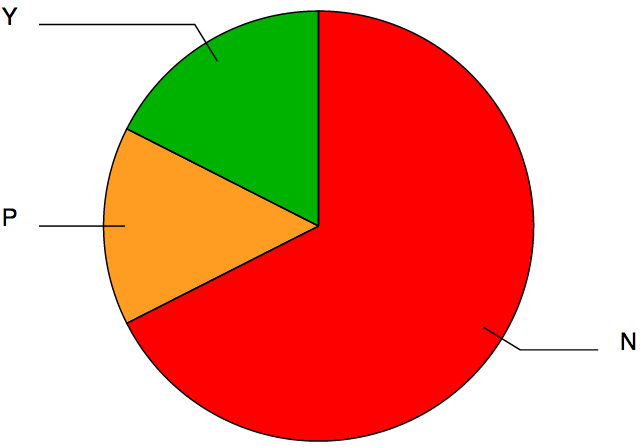
\includegraphics[width=0.55\linewidth]{figures/toolsavailability}
            %\end{figure}
        \end{frame}

        \subsection{Why Important?}
        \begin{frame}
            \frametitle{Scenario 1: MSR Tool Building and Sharing}
        User wants to build a tool for Association Mining
        %    Build    a tool for mining the source code, version data, and bugs
            \begin{columns}
                \column{0.65\textwidth}
                    \begin{itemize}
                      \item Source code
                          \begin{itemize}
                            \item Java source code
                          \end{itemize}
                      \item Version control systsm(VCS)
                          \begin{itemize}
                            \item GIT
                          \end{itemize}
                      \item Bug Information
                          \begin{itemize}
                            \item Github-Issues Bug Tracker
                          \end{itemize}
                    \end{itemize}

                \column{0.35\textwidth}
                    \begin{figure}
                    \centering
                    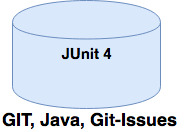
\includegraphics[width=0.60\linewidth]{figures/junit4.jpg}
                    \caption{\tiny{Software Repository Data}}
                    \end{figure}

            \end{columns}
        \end{frame}

        \begin{frame}
            \frametitle{Scenario 1: Tool Building and Sharing}
            Build a tool for association mining
            \begin{figure}
                \centering
                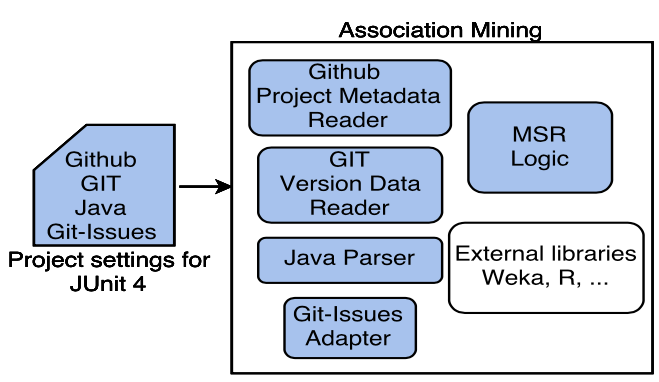
\includegraphics[width=0.60\linewidth]{figures/association.png}
                \caption{Association Minging Tool Details}
            \end{figure}
        \end{frame}

        \begin{frame}
            \frametitle{Scenario 1: Tool Building and Sharing}
            Share the built tool with other researchers and practitioners
            \begin{figure}
                \centering
                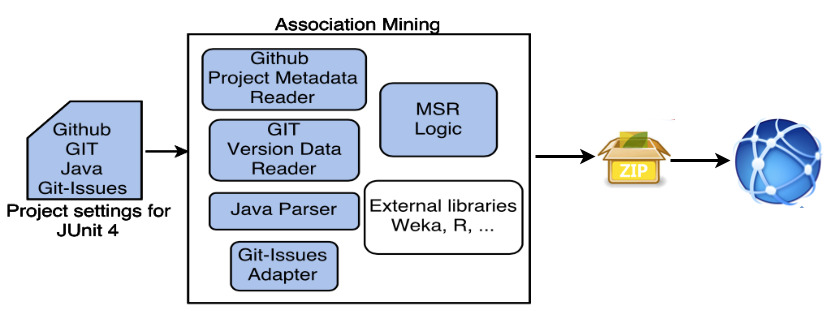
\includegraphics[width=0.85\linewidth]{figures/junitsharing.jpg}
                \caption{Complete process of building and sharing tool}
            \end{figure}
        \end{frame}

        \begin{frame}
            \frametitle{Scenario 2: Adopting a shared tool}
            \begin{figure}
                \centering
                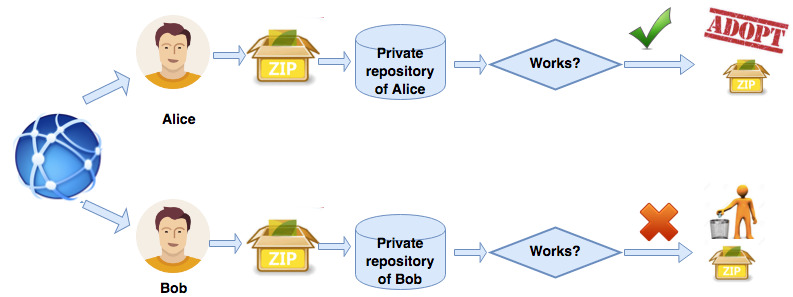
\includegraphics[scale=0.35]{figures/adopting.jpg}
                \caption{Repository Mining Tool Building}
            \end{figure}
        \end{frame}

%\begin{comment}
        \begin{frame}
            \frametitle{Scenario 2: Adopting a shared MSR tool}
             \centering
                Why Bob is not able to adopt the same tool? \\
                \& \\
                What are the possible points of failure?
        \end{frame}
%\end{comment}

        \begin{frame}
            \frametitle{How MSR tools are build?}
            \begin{itemize}
                \item MSR tools are build for specific project setting.
                \item A project setting defines types and sources of various MSR artifacts
            \end{itemize}
        \end{frame}

                \begin{frame}
                    \frametitle{How MSR tools are build?}
                    \begin{itemize}
                        \item MSR tools are build for specific project setting.
                        \item A project setting defines types and sources of various MSR artifacts
                        \item MSR Artifacts: Any kind of information realted to your software
                        \begin{itemize}
                            \item Revision history from version control system (VCS)
                            \item Source code of programming language(s)
                            \item Bug data from bug trackers
                            \item Project metadata
                            \item users and teams data from forges
                        \end{itemize}
                    \end{itemize}
                \end{frame}

        \begin{frame}
            \frametitle{Association Mining Tool Challenges}
            \begin{columns}
            %    Build    a tool for mining the source code, version data, and bugs
                \column{0.5\textwidth}
                \begin{itemize}
                    \item User is required to build necessary data preperation tools
                 \end{itemize}
                \column{0.65\textwidth}
                 \begin{figure}
                    \centering
                        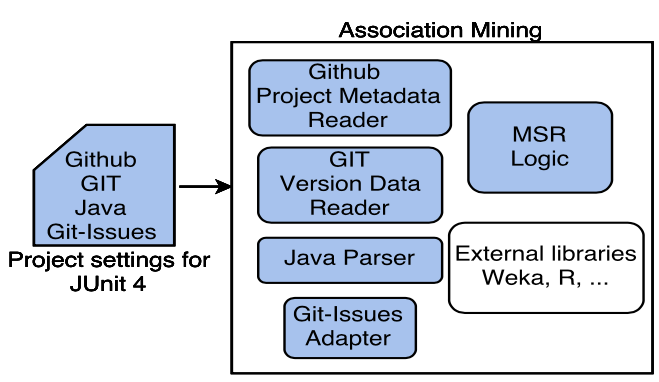
\includegraphics[width=0.85\linewidth]{figures/association.png}
     %                       \caption{Software Repository Data}
                 \end{figure}
             \end{columns}
        \end{frame}

        \begin{frame}
            \frametitle{Association Mining Tool Challenges}
            \begin{columns}
            %    Build    a tool for mining the source code, version data, and bugs
                \column{0.5\textwidth}
                \begin{itemize}
                    \item User is required to build necessary data preperation tools
                    \item Tool are tightly coupled with SCM systems
                 \end{itemize}
                \column{0.65\textwidth}
                 \begin{figure}
                    \centering
                        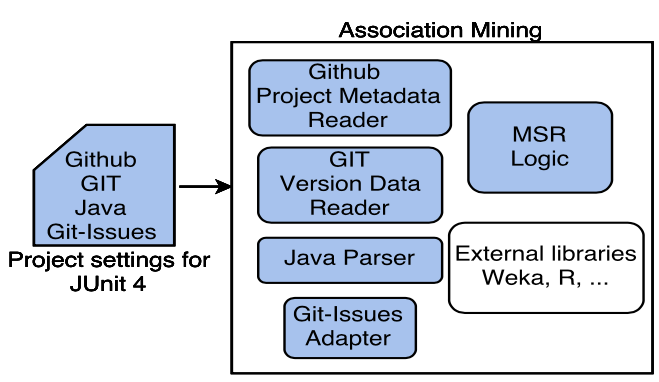
\includegraphics[width=0.85\linewidth]{figures/association.png}
     %                       \caption{Software Repository Data}
                 \end{figure}
             \end{columns}
        \end{frame}


        \begin{frame}
            \frametitle{Potential Points of failure}
            \begin{alertblock}{Failure Cause}
                An MSR tool build for one project setting may not work for different project settings.
            \end{alertblock}
             \begin{figure}
                \centering
                    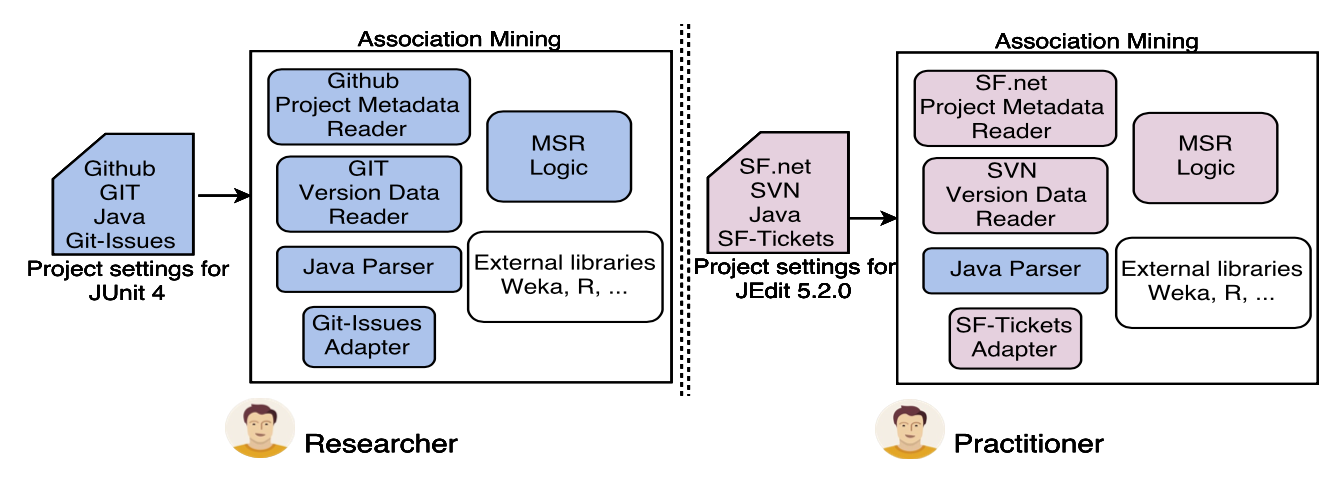
\includegraphics[width=0.85\linewidth]{figures/adoptingreserch.png}
                        \caption{A scenario of a practitioner adopting a MSR tool built by a researcher.}
             \end{figure}
        \end{frame}

\begin{comment}
        \begin{frame}
            \frametitle{Failure: Mismatched Project Settings}
             %    Build    a tool for mining the source code, version data, and bugs
             \begin{columns}
                \column{0.33\textwidth}
                    \centering Tool
                    \begin{figure}
                        \centering
                        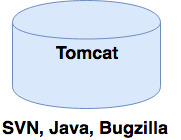
\includegraphics[width=0.45\linewidth]{figures/tomcat.jpg}
 %                       \caption{Software Repository Data}
                    \end{figure}

                \column{0.33\textwidth}
                    \centering Alice
                    \begin{figure}
                        \centering
                        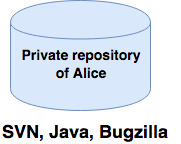
\includegraphics[width=0.45\linewidth]{figures/privaterepo.jpg}
%                        \caption{Software Repository Data}
                    \end{figure}

                \column{0.33\textwidth}
                    \centering Bob
                    \begin{figure}
                        \centering
                        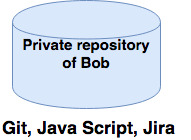
\includegraphics[width=0.45\linewidth]{figures/privaterepobob.jpg}
%                        \caption{Software Repository Data}
                    \end{figure}
             \end{columns}
        \end{frame}

    \subsection{A study of reusability of MSR tools}
        \begin{frame}
            \frametitle{Reusability of published MSR tools\footnote{\label{replicability}{Replicating MSR:A study of the potential replicability of papers, Gregorio Robles et.al,  MSR 2010}}}
            \begin{columns}
                \column{0.55\textwidth}
                    \centering
                        \begin{itemize}
                            \item Y = Replicable
                            \item N = Not replicable
                            \item P = Partially replicable
                        \end{itemize}

                \column{0.45\textwidth}
                    \centering
                    \begin{figure}
                        \centering
                        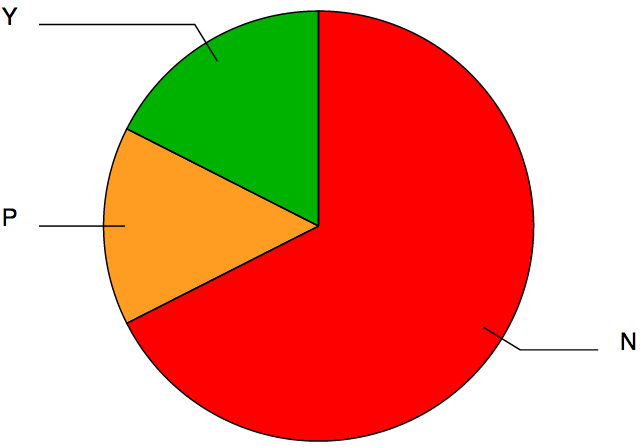
\includegraphics[width=0.75\linewidth]{figures/toolsavailability.png}
                        \caption{Replicability of $MSR^{3}$}
                    \end{figure}
            \end{columns}
        \end{frame}

\end{comment}

        \begin{frame}
            %\frametitle{Challenges: Scenario 1 MSR Tool Building and Sharing}
        %    Build    a tool for mining the source code, version data, and bugs
             \centering
             How to make adopting MSR tools possible?
        \end{frame}
  \section{Solution}
    \subsection{Solution Overview}
        \begin{frame}
        \frametitle{Our Solution}
        \begin{itemize}
          \item Software As Apps
            \begin{itemize}
                \item Make tool size smaller by pushing generic functionality in the platform
            \end{itemize}
          \item Programs as Script
            \begin{itemize}
                \item Make tool components more like scripts, than programs, easier to customize
            \end{itemize}
          \item Platform and appstore
            \begin{itemize}
                \item Provide a platform and ecosystem to distribute these tools
            \end{itemize}

        %  deterministic \textbf{transformations} (\texttt{map}, \texttt{filter}, \texttt{join}, \ldots)
        %  \item \textbf{Actions} (\texttt{count}, \texttt{collect}, \texttt{reduce},
        %  \ldots) either return value or write to storage
        \end{itemize}
        \end{frame}

        \begin{frame}
            \frametitle{How to build Software as Apps?}
            \begin{figure}
                \centering
                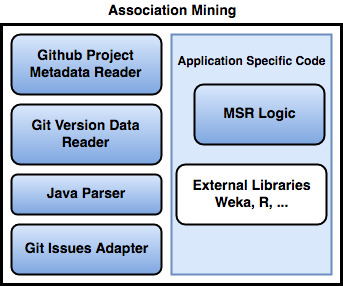
\includegraphics[scale=0.30]{figures/association.jpg}
                \caption{An MSR Tool Structure}
            \end{figure}
        \end{frame}

        \begin{frame}
            \frametitle{Pull supporting tools out and make them available as part of platform}
            \begin{figure}
                \centering
                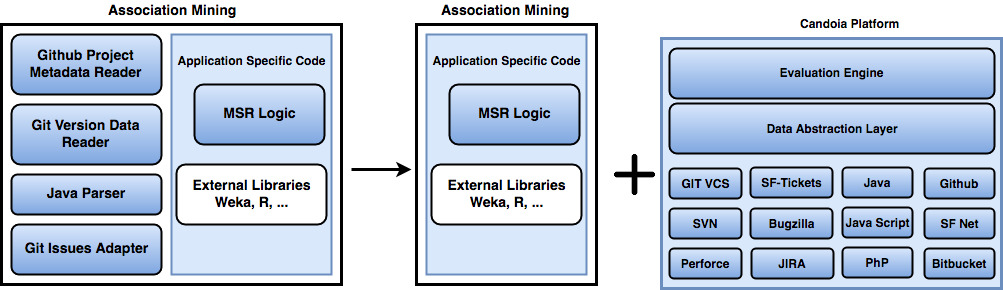
\includegraphics[width=0.75\linewidth]{figures/candoia_idea_overview.jpg}
                \caption{Repository Mining Tool Building}
            \end{figure}
        \end{frame}


        \begin{frame}
            \frametitle{How to build programs as Script?}
            \begin{figure}
                \centering
                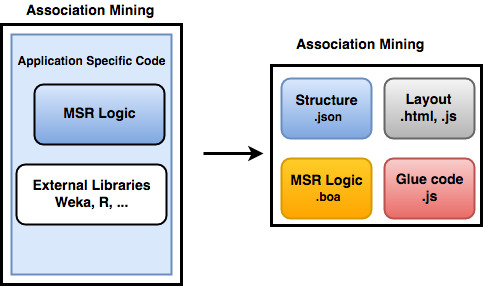
\includegraphics[scale=0.25]{figures/programtoscript.jpg}
                \caption{Transofrmation of MSR program to MSR tool}
            \end{figure}
        \end{frame}

        \begin{frame}
            \frametitle{MSR Tool as Candoia App}
            \begin{figure}
                \centering
                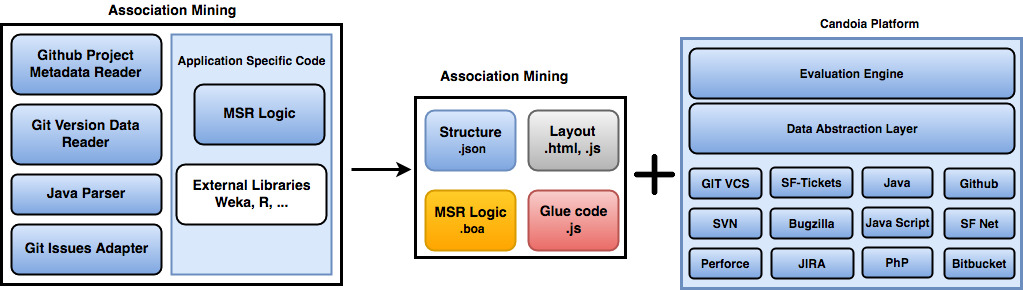
\includegraphics[width=0.75\linewidth]{figures/programstoscriptincandoia.jpg}
                \caption{MSR tool to Candoia App transformation}
            \end{figure}
        \end{frame}

        \begin{frame}
            \frametitle{Process Of Building and Sharing Candoia App}
            \begin{figure}
                \centering
                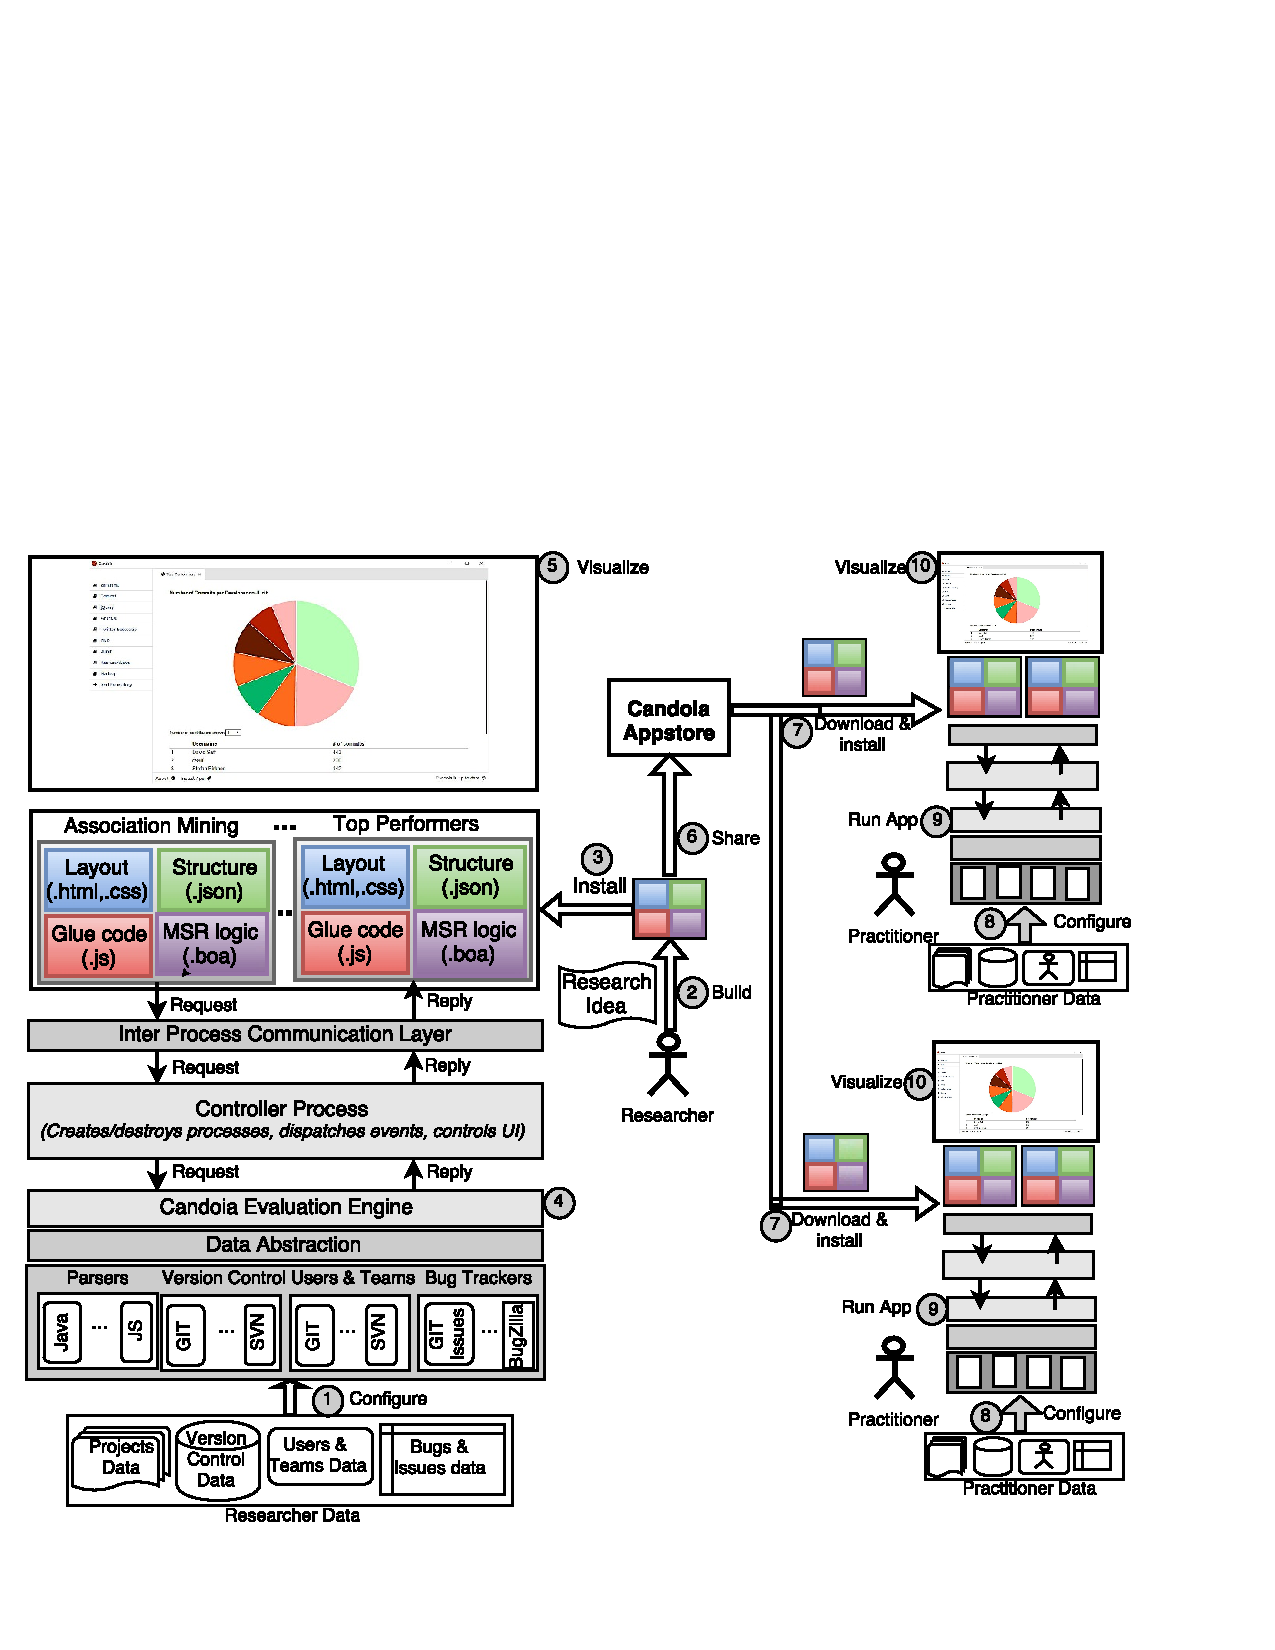
\includegraphics[width=0.6\linewidth]{figures/overview.pdf}
%                \caption{Repository Mining Tool Building}
            \end{figure}
        \end{frame}


    \subsection{Candoia Apps}
        \begin{frame}
        \frametitle{Candoia App Structure}
        \begin{columns}
            \column{0.45\textwidth}
                \begin{itemize}
                  \item Mining Logic
                    \begin{itemize}
                        \item Extension of Boa DSL
                    \end{itemize}
                  \item Visualization Layout
                    \begin{itemize}
                        \item Html
                        \item CSS
                    \end{itemize}
                  \item Glue Code
                    \begin{itemize}
                        \item Java script
                    \end{itemize}
                  \item Structure Decription
                    \begin{itemize}
                        \item Json %(file package.json)
                    \end{itemize}
                \end{itemize}

            \column{0.65\textwidth}
                \begin{figure}
                    \centering
                    
\includegraphics[scale=0.28]{figures/structure.png}
                    \caption{Structure of an Candoia app}
                \end{figure}
        \end{columns}
        \end{frame}

     \subsection{Data Abstraction}
        \begin{frame}
        \frametitle{Data Abstraction}
            \begin{itemize}
                \item Queries are written over data abstractions
               \item Data abstractions provide capability of running an app over data collected
               from diverse sources
               \item Candoia's data abstraction is extension of Boa DSL.
            \end{itemize}
        \end{frame}


        \begin{frame}
        \frametitle{Candoia Data Schema}
                \begin{figure}
                    \centering
                    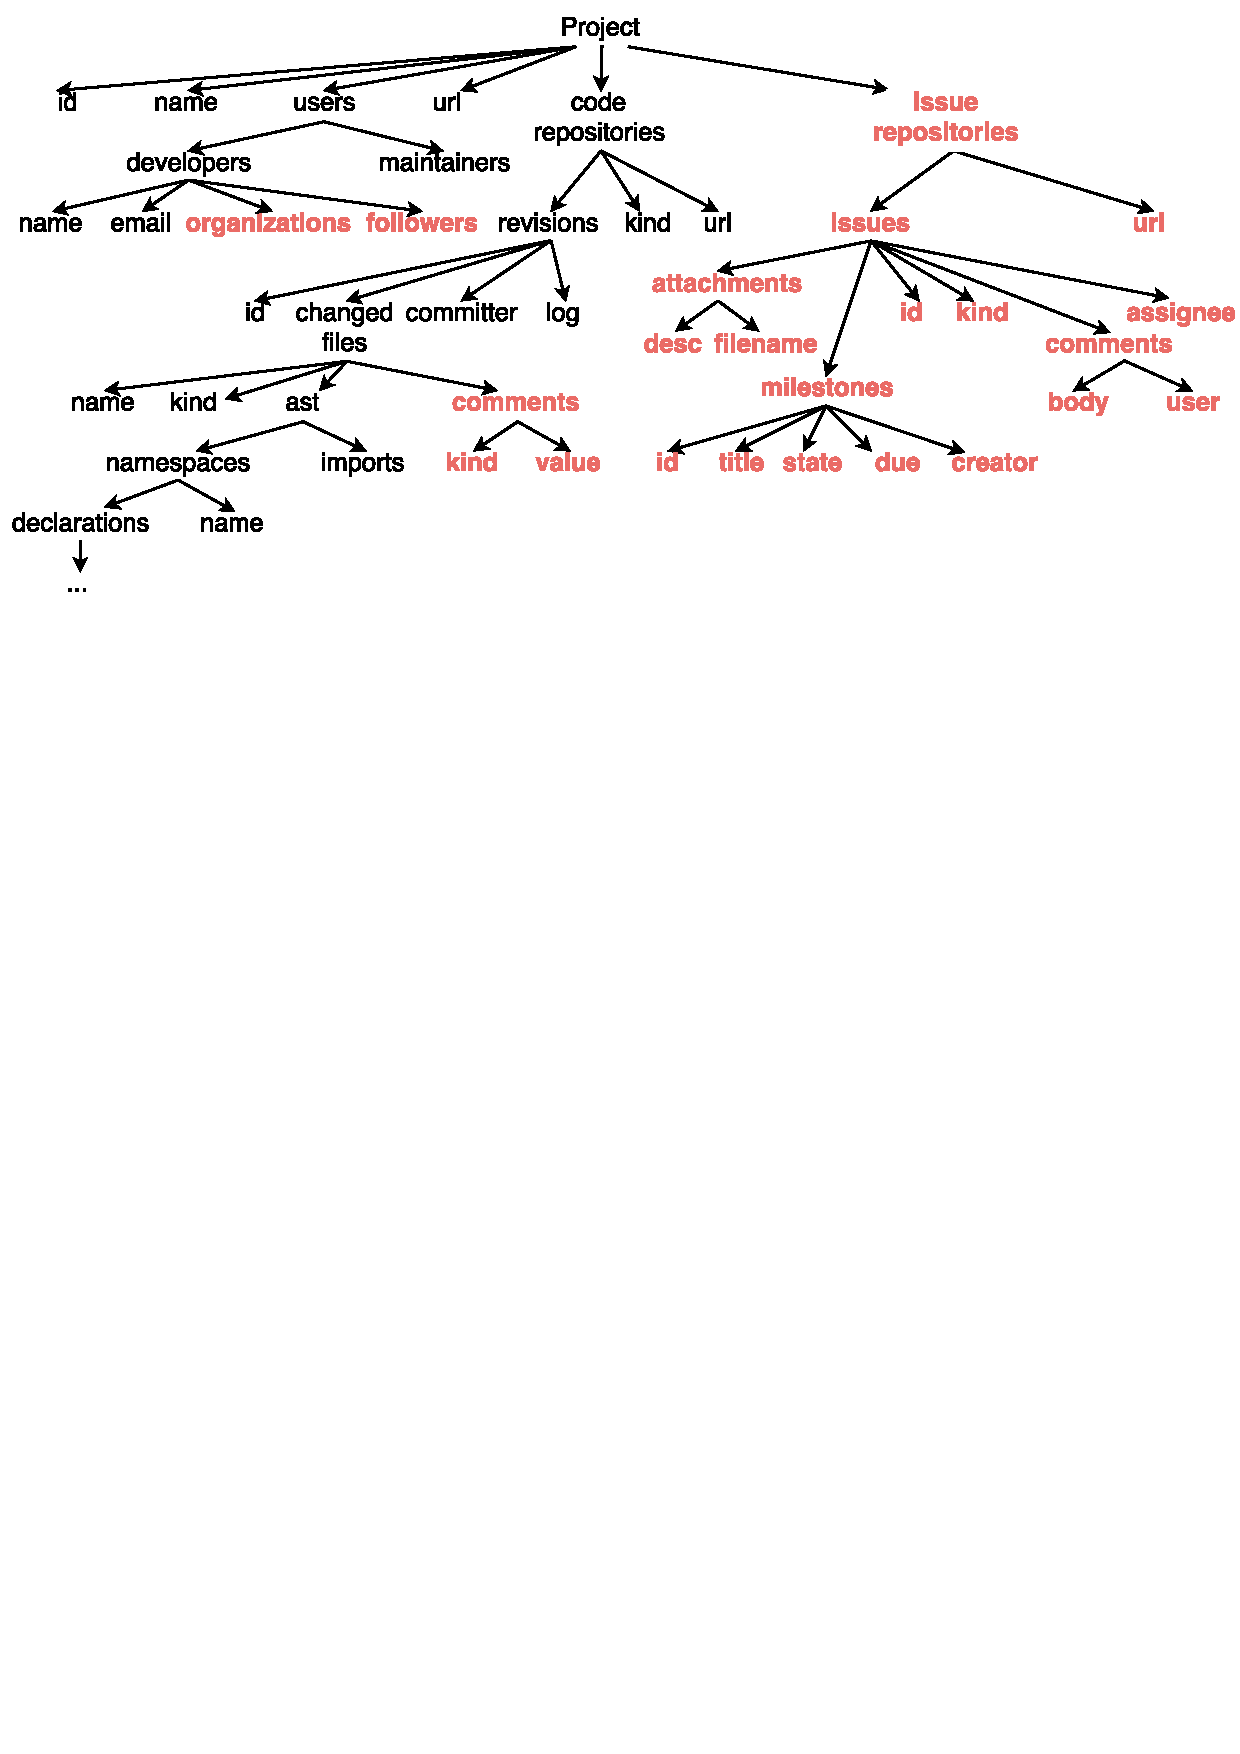
\includegraphics[scale=0.45]{figures/data-schema.pdf}
                    \caption{Candoia's data schema}
                \end{figure}
        \end{frame}

    \subsection{Customization}
        \begin{frame}
        \frametitle{Customizations}
            Two levels of customizations
            \begin{itemize}
                \item Data source customizations
                \item App Customization
            \end{itemize}
        \end{frame}

        \begin{frame}
        \frametitle{Customizations}
            Two levels of customizations
            \begin{itemize}
                \item Data source customizations
                    \begin{itemize}
                        \item Concerned with changing the source of the data
                        \item No Change in app required
                        \item Just rerun the application with new datasource
                    \end{itemize}
                \item Customization in Apps
            \end{itemize}
        \end{frame}

        \begin{frame}
        \frametitle{Customizations}
            Two levels of customizations
            \begin{itemize}
                \item Data source customizations
                \item Customization in Apps
                    \begin{itemize}
                        \item Concerned with customizing different part of the apps
                        \item App customizations in Candoia are more focused in terms of findings the right component(s) for customizations
                    \end{itemize}
            \end{itemize}
        \end{frame}

        \begin{frame}
        \frametitle{Customizations}
            Two levels of customizations
            \begin{itemize}
                \item Data source customizations
                \item Customization in Apps
                    \begin{itemize}
                        \item Concerned with customizing different part of the apps
                        \item app customizations in Candoia are more focused in terms of findings the right component(s) for customizations
                        \end{itemize}
            \begin{figure}
                \centering
                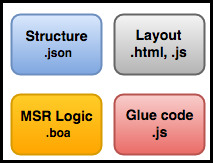
\includegraphics[scale=0.40]{figures/app.jpg}
                \caption{An MSR App Structure}
            \end{figure}
            \end{itemize}
        \end{frame}


        \begin{frame}
        \frametitle{Customizations}
            Two levels of customizations
            \begin{itemize}
                \item Data source customizations
                \item Customization in Apps
                    \begin{itemize}
                        \item Concerned with customizing different part of the apps
                        \item App customizations in Candoia are more focused in terms of findings the right component(s) for customizations
                        \item Script based app, easire to customize
                    \end{itemize}
            \end{itemize}
        \end{frame}


    \subsection{Evaluation Engine}
        \begin{frame}
            \frametitle{Candoia Evaluation Engine}
            \begin{itemize}
                \item Interpreter based Query evaluator for extended Boa DSL
            \end{itemize}
        \end{frame}

    \subsection{Evaluation Engine}
        \begin{frame}
            \frametitle{Candoia Evaluation Engine}
            \begin{itemize}
                \item Interpreter based Query evaluator of extended Boa DSL
                \item Reads data from local and remote software artifacts
                    \begin{itemize}
                        \item Forges: Github, Source Forge
                        \item VCS: GIT, SVN
                        \item Bug Tracker: Bugzilla, JIRA, Github-Issue, SF-Ticket
                        \item Programming Language: Java, Javascript
                    \end{itemize}
                \end{itemize}
            \end{frame}


    \subsection{Evaluation Engine}
        \begin{frame}
            \frametitle{Candoia Evaluation Engine}
            \begin{itemize}
                \item Interpreter based Query evaluator of extended Boa DSL
                \item Reads data from local and remote software artifacts
                    \begin{itemize}
                        \item Forges: Github, Source Forge
                        \item VCS: GIT, SVN
                        \item Bug Tracker: Bugzilla, JIRA, Github-Issue, SF-Ticket
                        \item Programming Language: Java, Javascript
                    \end{itemize}
                \item Process level parallelization for running multiple apps
                \item Thread level prarallelization for dataset creation
                \item Provides fine grained control to Candoia frontend
                \end{itemize}
            \end{frame}



    \subsection{Security Architecture}
        \begin{frame}
            \frametitle{Candoia Security Concern}
            \begin{itemize}
                \item Private software data
                    \begin{itemize}
                        \item Allow access to user data on a need to know basis
                    \end{itemize}
                \item Installing and running third party apps
                    \begin{itemize}
                        \item Prevent apps from corrupting each other
                        \item Prevent apps from accessing system resources directly
                    \end{itemize}
            \end{itemize}
         \end{frame}

        \begin{frame}
            \frametitle{Chromium based Candoia frontend}
            \begin{itemize}
                \item Candoia builds on the process architecture of Chromium, each window runs as a process
                \item Process communica tes with controller process via Inter Process Communication
                \item Controller process mediates interaction between file system, window data etc. by exposing APIs.
                \item An app can only access resources using exposed APIs.
            \end{itemize}
         \end{frame}

        \begin{frame}
            \frametitle{Few APIs available to Candoia app}
            \begin{itemize}
                \item Running MSR queries (api.boa)
                \item Reading (not writing) files within app (api.fs)
                \item Saving arbitrary data between instances (api.store)
                \item Getting its own package info such as version (api.meta)
                \item Inter-Process-Communication handle (api.ipc)
%                \item Using pre-made views/graphs. (api.view)
            \end{itemize}
            \centering
                \emph{var data = api.boa.run('myprog.boa')}
         \end{frame}

        \begin{frame}
            \frametitle{Candoia Exchange}
            \begin{itemize}
                \item A web platform for sharing MSR apps
                \item Candoia frameworks can connect to exchange for gathering information and  installing apps
            \end{itemize}
         \end{frame}
%  \section{Spark Internals}

\subsection{Example walk-through}
\begin{frame}
\begin{figure}
\centering
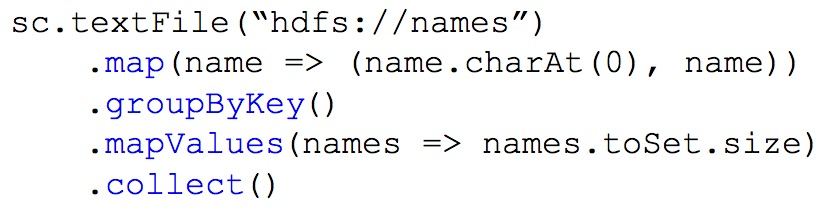
\includegraphics[width=0.8\linewidth]{figures/example2.jpg}
\caption{Find number of distinct names per ``first letter''. This example is
reproduced from [3].}
\end{figure}
\end{frame}

\begin{frame}
\begin{figure}
\centering
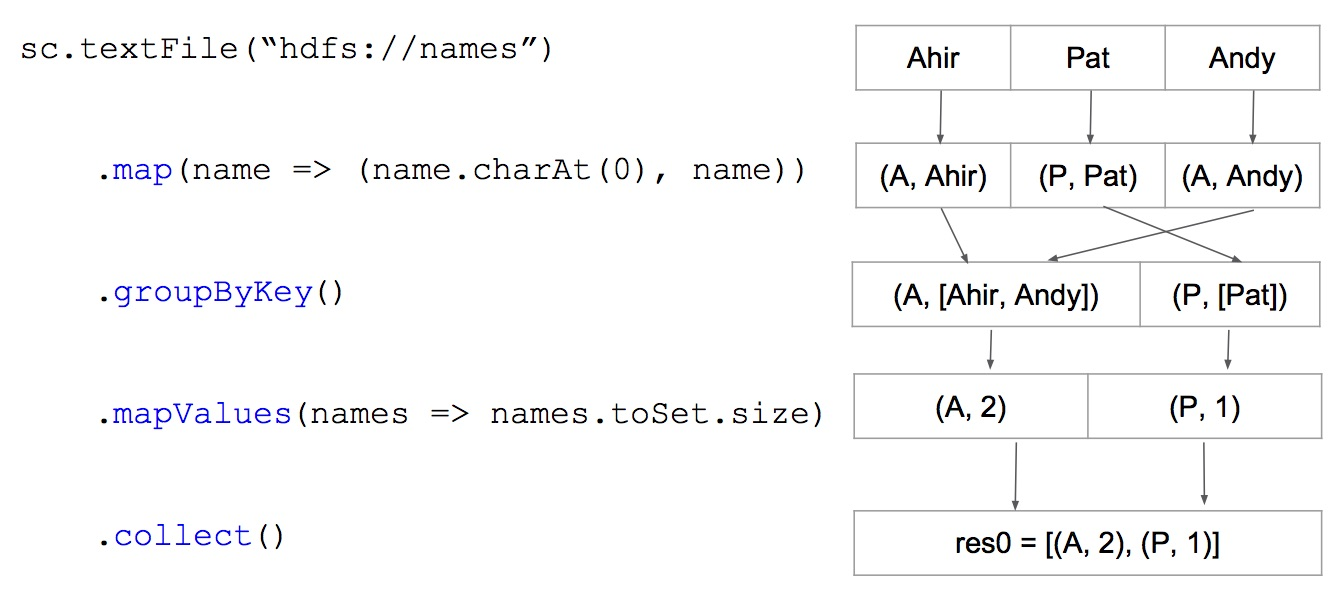
\includegraphics[width=0.9\linewidth]{figures/example2-wall-through.jpg}
\end{figure}
\end{frame}

\subsection{Lineage of RDDs}
\begin{frame}
\begin{figure}
\centering
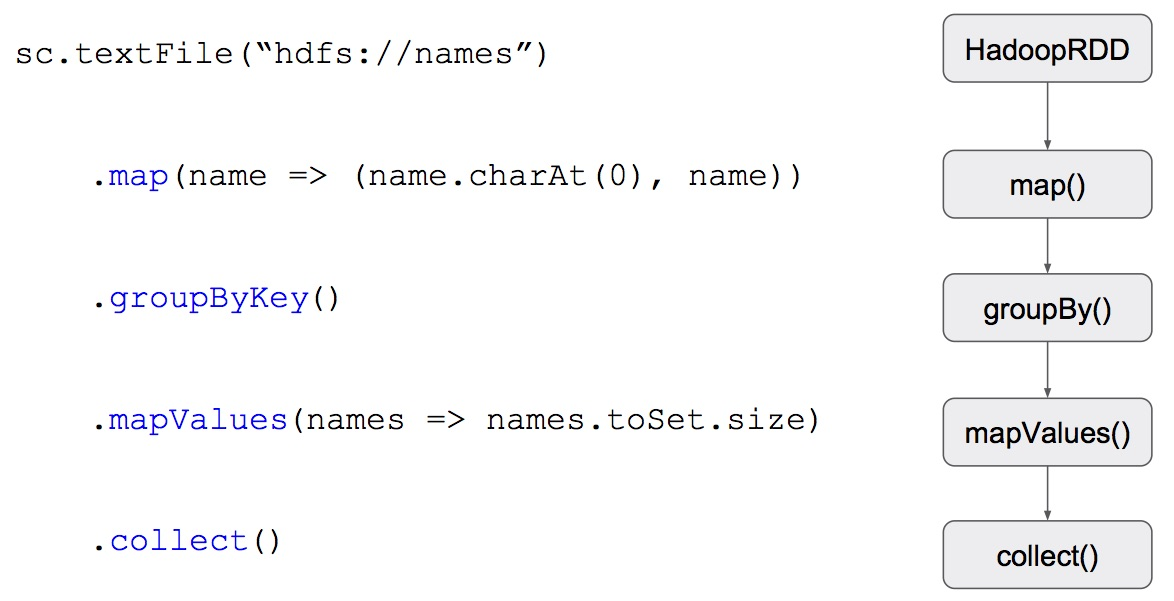
\includegraphics[width=0.9\linewidth]{figures/example2-rdd-dag.jpg}
\end{figure}
\end{frame}

\subsection{Staging}
\begin{frame}
\begin{figure}
\centering
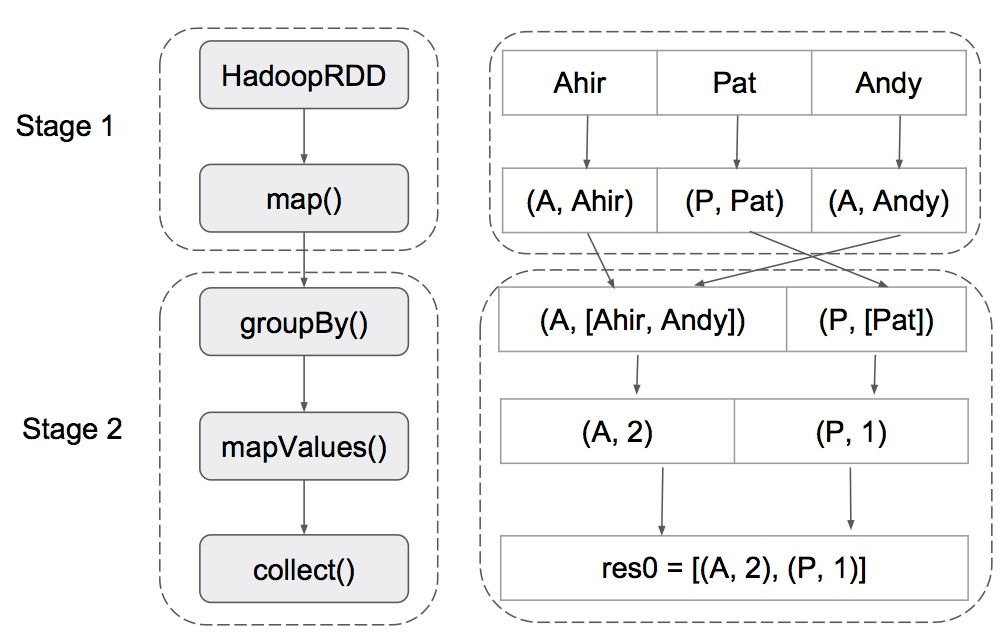
\includegraphics[width=0.6\linewidth]{figures/example2-staging.jpg}
\end{figure}
\end{frame}

\subsection{Execution Model}
\begin{frame}
\begin{figure}
\centering
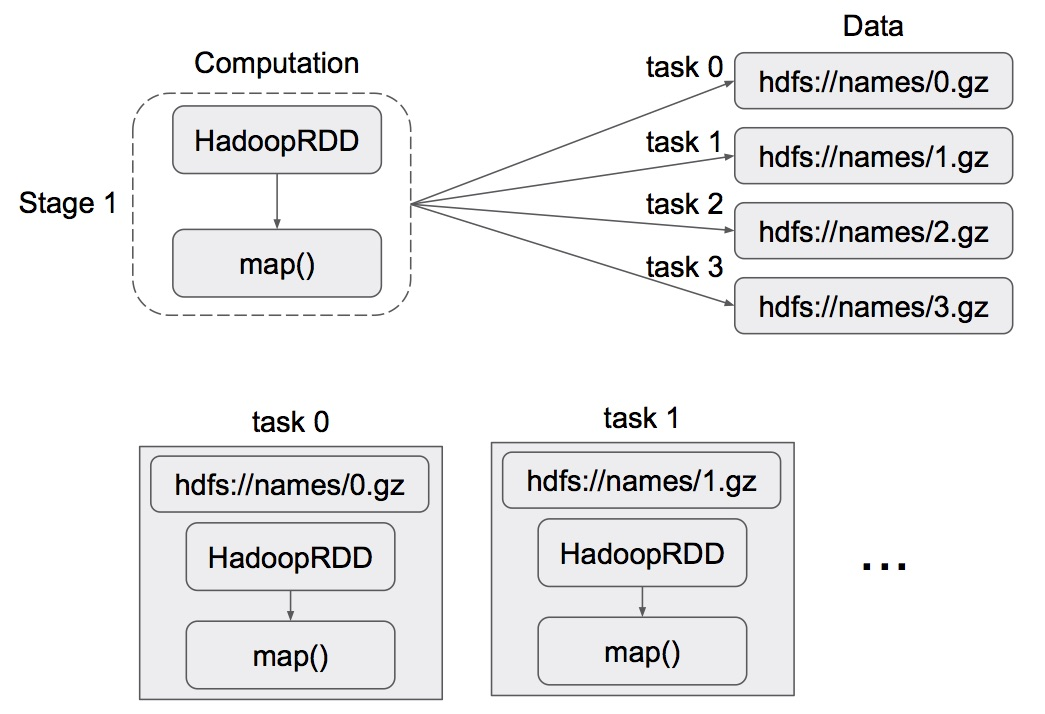
\includegraphics[width=0.8\linewidth]{figures/example2-tasking.jpg}
\end{figure}
\end{frame}

\subsection{Scheduling}
\begin{frame}
\begin{figure}
\centering
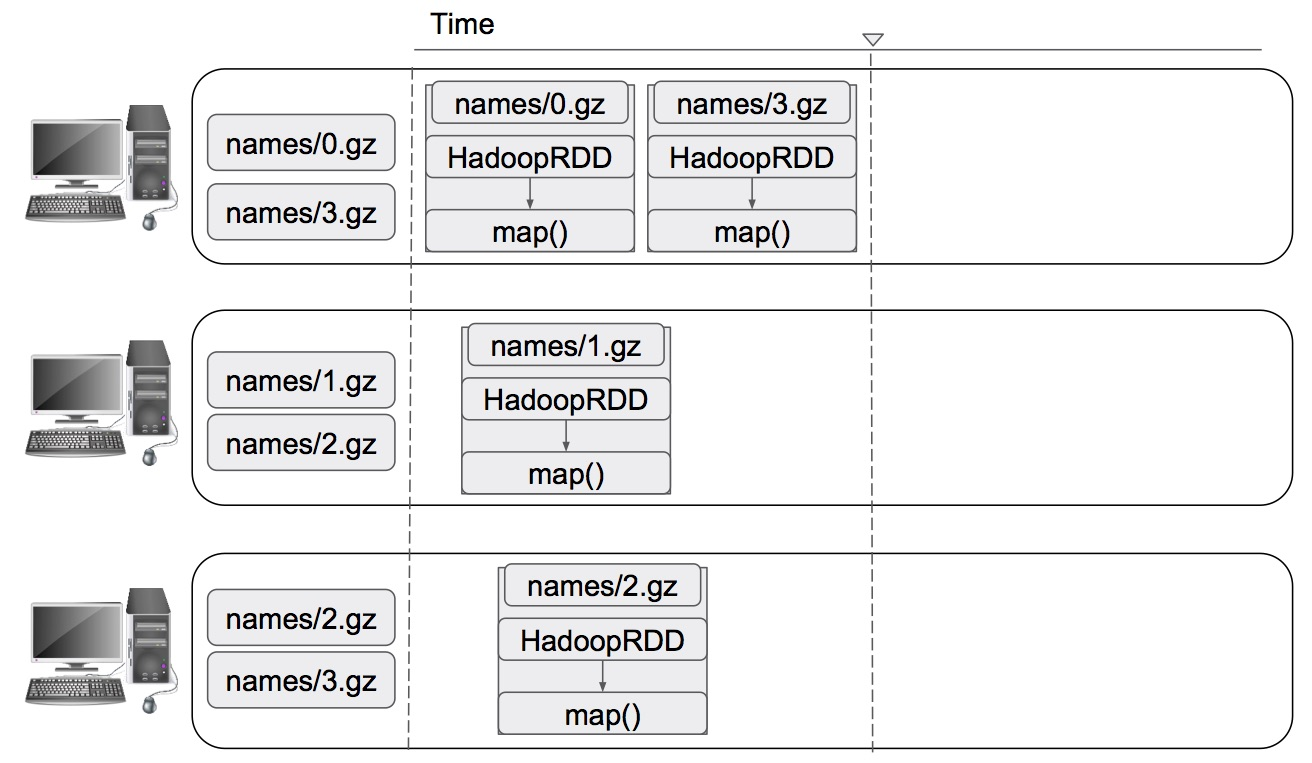
\includegraphics[width=0.9\linewidth]{figures/example2-scheduling.jpg}
\end{figure}
\end{frame}

\subsection{Shuffling}
\begin{frame}
\begin{figure}
\centering
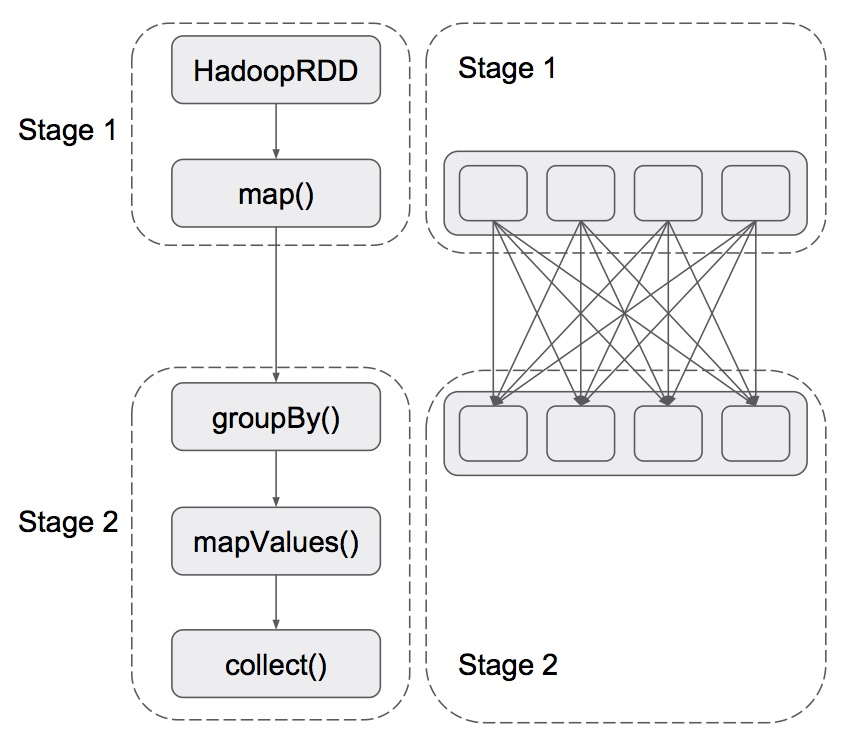
\includegraphics[width=0.6\linewidth]{figures/example2-shuffling.jpg}
\end{figure}
\end{frame}


\begin{frame}
\begin{figure}
\centering
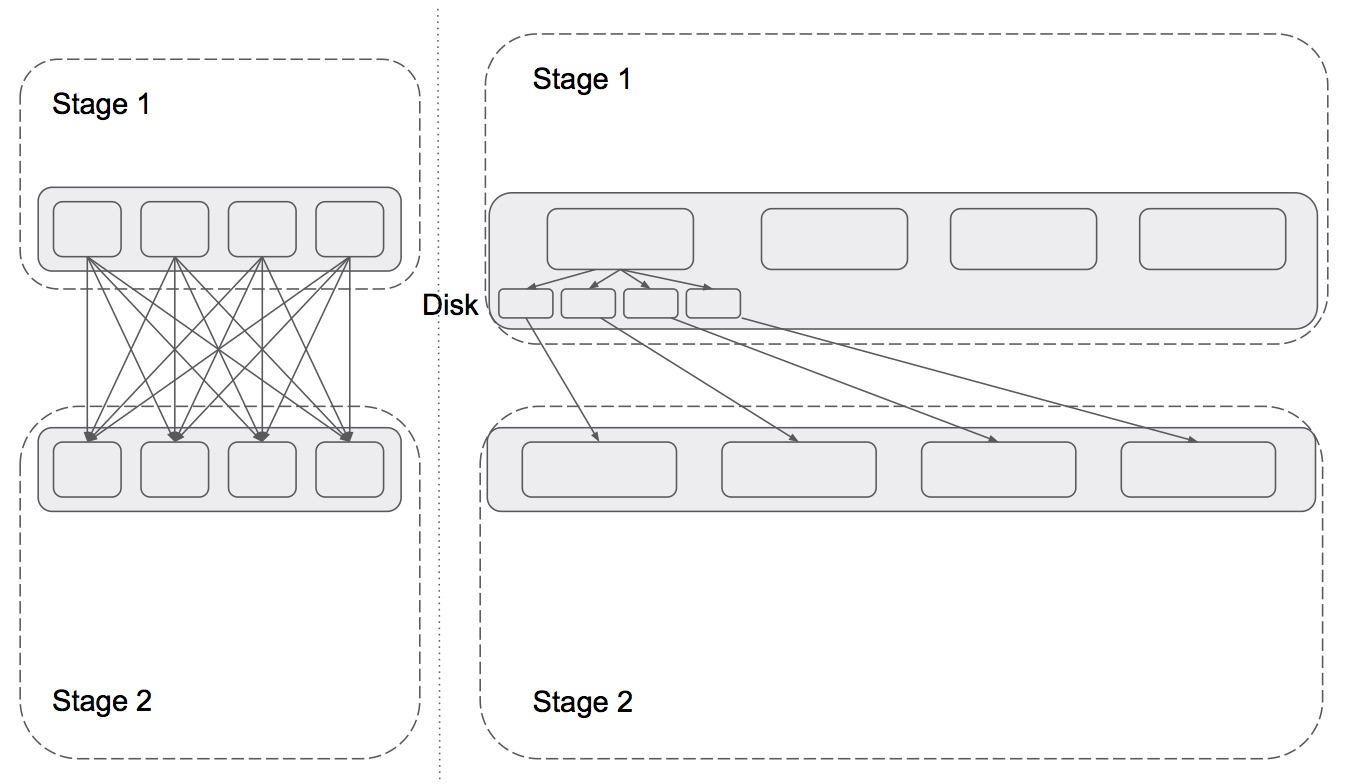
\includegraphics[width=0.9\linewidth]{figures/example2-shuffling-details.jpg}
\end{figure}
\end{frame}
%  \section{RDDs Essentials}

\subsection{Examples}
\begin{frame}[fragile]
\begin{lstlisting}
	val data = Array(1, 2, 3, 4, 5)
	val distData = sc.parallelize(data)
	
	// add up the elements of the array
	distData.reduce((a, b) => a + b)
	
	// specify number of partitions
	// default: sets automatically based on cluster
	// runs one task for each partition of the cluster
	distData = sc.parallelize(data, 10) 
	
	val distFile = sc.textFile("data.txt")
	
	// add up the sizes of all the lines
	distFile.map(s => s.length).reduce((a, b) => a + b)
	
	// passing functions
	object MyFunctions { def func1(s: String): String = { ... } }
	myRdd.map(MyFunctions.func1)
\end{lstlisting}
\end{frame}

\subsection{Local vs. Cluster}
\begin{frame}[fragile]
\begin{lstlisting}
	var counter = 0
	var rdd = sc.parallelize(data)
	rdd.foreach(x => counter += x)	
	println("Counter value: " + counter)
\end{lstlisting}
\begin{itemize}
  \item Behavior of the above code is undefined
  \item In local mode, works because counter is in the memory of driver
  \item In cluster mode, a new copy of counter is sent to each node in the
  cluster,
  \item In cluster mode, use accumulators to make it work.
  \item Closure: those variables and methods which must be visible for the
  executor to perform its computations on the RDD
  \item The closure is serialized and sent to each executor
\end{itemize}
\end{frame}

\begin{frame}[fragile]
Spark supports ``Shared Variables'' along with RDDs
\begin{itemize}
  \item closure (variable + function) runs in parallel as set of tasks in nodes
  \item generally ships copy of each variable to each task
  \item for sharing across tasks: i) broadcast variables, ii) accumulators
  \item broadcast: cache a value in memory on all nodes
  \item accumulators: variables that are only ``added'', e.g., counters, sums.
\end{itemize}
\begin{lstlisting}
	val broadcastVar = sc.broadcast(Array(1, 2, 3))
	
	val accum = sc.accumulator(0, "My Accumulator")
	sc.parallelize(Array(1, 2, 3, 4)).foreach(x => accum += x)
\end{lstlisting}
\end{frame}

\subsection{RDD Operations}
\begin{frame}
\begin{figure}
\centering
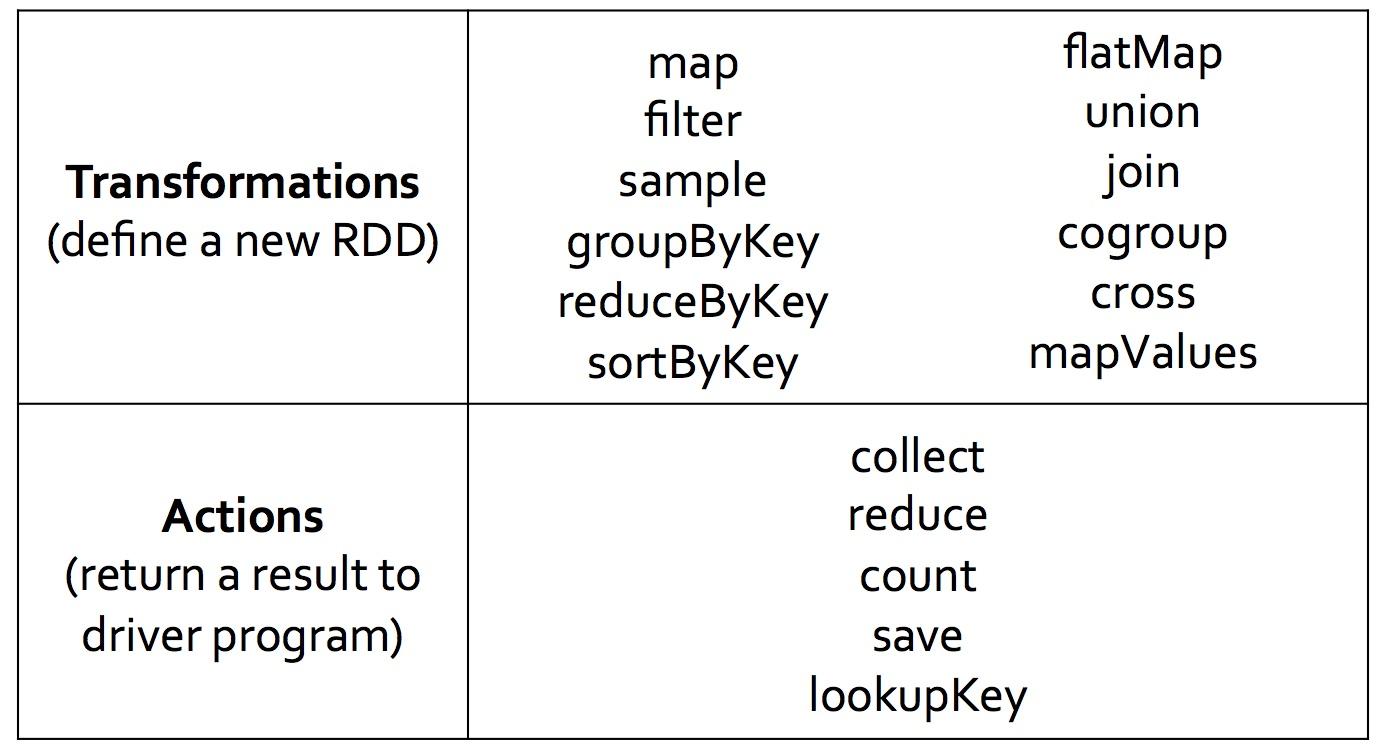
\includegraphics[width=0.80\linewidth]{figures/rdd-operations.jpg}
\caption{Transformations and actions available on RDDs in Spark [2].}
\end{figure}
\end{frame}

\begin{frame}
\begin{figure}
\centering
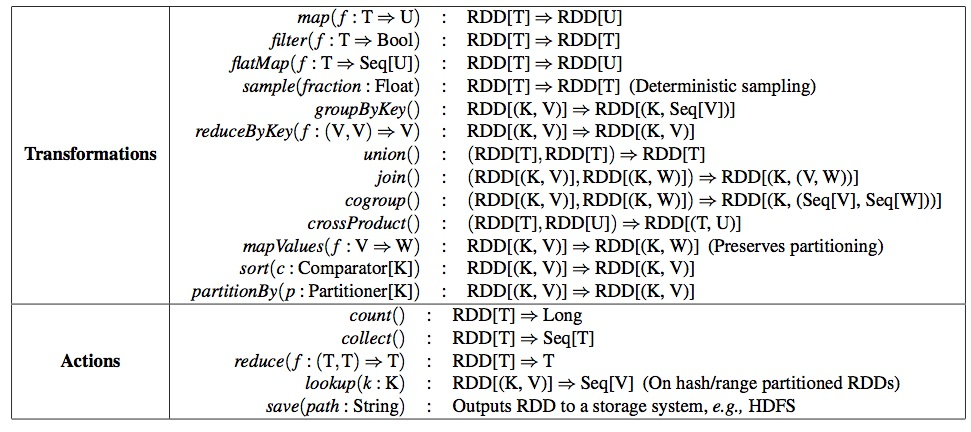
\includegraphics[width=\linewidth]{figures/rdd-operations-details.jpg}
\caption{Transformations and actions available on RDDs in Spark [1].}
\end{figure}
\end{frame}

\subsection{RDD Persistence}
\begin{frame}
\begin{itemize}
  \item Persist RDDs using \texttt{persist()} or \texttt{cache()}
  \item Persisted RDDs can be stored using a storage level
  \item \textit{MEMORY\_ONLY} (default): store RDD as deserialized Java object
  in the JVM, RDD partitions that don't fit will be recomputed
  \item \textit{MEMORY\_AND\_DISK}: similar to before but stores the partitions
  that don't fit on disk
  \item \textit{MEMORY\_ONLY\_SER}: store RDD as serialized Java object
  \item \textit{MEMORY\_AND\_DISK\_SER}: similar but store on disk too
  \item \textit{DISK\_ONLY}: store the RDD partitions only on disk
\end{itemize}
\end{frame}

\begin{frame}
Which storage level to choose?
\begin{itemize}
  \item if RDD fits comfortably with default, leave it as is
  \item if not, try \textit{MEMORY\_ONLY\_SER} and select fast serialization
  library
  \item don't spill to disk unless the functions that computed datasets are
  expensive (otherwise recomputing may be as fast as reading from disk)
  \item use replicated storage level for faster fault recovery
  \item spark automatically monitors cache usage on each node and drops out old
  partitions based on LRU. For manual, \texttt{RDD.unpersist()}
\end{itemize}
\end{frame}

\subsection{RDD Representation}
\begin{frame}
\begin{figure}
\centering
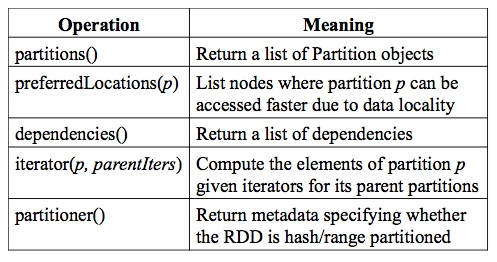
\includegraphics[width=0.55\linewidth]{figures/rdd-representation.jpg}
\end{figure}
RDD interface exposes five pieces of information:
\begin{itemize}
  \item a set of \textit{partitions}, which are atomic pieces of the dataset 
  \item a set of \textit{dependencies} on parent RDDs
  \item a function for computing the dataset based on its parents
  \item metadata about its partitioning
  \item metadata about its data placement
\end{itemize}
\end{frame}

\begin{frame}
Dependencies,
\begin{figure}
\centering
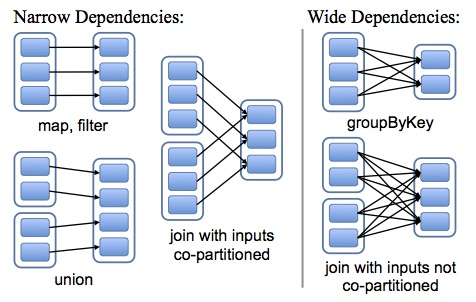
\includegraphics[width=0.45\linewidth]{figures/rdd-dependies.jpg}
\caption{Narrow and wide dependencies [1].}
\end{figure}
%\vpsace{-0.5cm}
Dependencies are useful for,
\begin{itemize}
  \item for staging (seen before, \texttt{groupByKey()})
  \item recovery after node failure, easy with narrow and difficult with wide.
\end{itemize}
\end{frame}


      \section{Evaluation}
    \subsection{Evaluation Critera}
        \begin{frame}
            \frametitle{Evaluation}
            \begin{itemize}
                \item Applicability
                    \begin{itemize}
                        \item Our claim is that MSR tasks and hypotheses can be expressed and evaluated using Candoia platform\'s capabilities.
                    \end{itemize}
                \item Adoptability
                    \begin{itemize}
                        \item Candoia apps are portable across diverse project settings and require no changes
                    \end{itemize}
                \item Customizability
                    \begin{itemize}
                        \item Our claim that performing customizations in Candoia requires less efforts in terms of LOC.
                    \end{itemize}
            \end{itemize}
         \end{frame}

        \begin{frame}
            \frametitle{Projects used in Evaluation}
            \begin{figure}[ht!]
\centering
% Please add the following required packages to your document preamble:
% \usepackage[table,xcdraw]{xcolor}
% If you use beamer only pass "xcolor=table" option, i.e. \documentclass[xcolor=table]{beamer}
%\resizebox{0.99\textwidth}{!}{%
% \small
\begin{adjustbox}{max width=0.9\textwidth}
\begin{tabular}{|
>{\columncolor[HTML]{C0C0C0}}l |l|l|l|r|r|r|r|}
\hline
Projects        &
\multicolumn{1}{c|}{\cellcolor[HTML]{C0C0C0}VCS} &
\multicolumn{1}{c|}{\cellcolor[HTML]{C0C0C0}PL}   &
\multicolumn{1}{c|}{\cellcolor[HTML]{C0C0C0}Bugs} &
\multicolumn{1}{c|}{\cellcolor[HTML]{C0C0C0}\#LOC} & 
\multicolumn{1}{c|}{\cellcolor[HTML]{C0C0C0}\#Revs} & 
\multicolumn{1}{c|}{\cellcolor[HTML]{C0C0C0}\#Bugs} & 
\multicolumn{1}{c|}{\cellcolor[HTML]{C0C0C0}\#Devs} \\
\hline 
Tomcat 8.0.24 (TC)  & SVN  & Java  & Bugzilla & 381350 & 17433 & 3023 & 32 \\
\hline

Hadoop 2.7.1 (HD)   & Git  & Java  & JIRA     & 2217636 & 14301 & 10333 & 146 \\ \hline

JUnit 4  (JU)       &Git   & Java  & GitHub   & 30535  & 2115  & 148  & 127 \\ \hline

SLF4j 1.7.12 (SLF)  & Git  & Java  & JIRA     & 20866  & 1436 & 332 & 59 \\ \hline

Bootstrap 3.3.5 (BT)& Git  & JS    & GitHub   & 65885 & 11840  & 213  & 718 \\
\hline

Node.js 0.12.7 (ND) & Git  & JS    & GitHub   & 3405739 & 14695   & 955 & 105 \\
\hline

Grunt 0.4.6  (GT)   & Git  & JS    & GitHub   & 3596 & 1399 & 155 & 29 \\ \hline

JQuery 2.1.4 (JQ)   & Git  & JS    & GitHub   & 45212  & 6153  & 165  & 87 \\
\hline

PMD 5.3.3 (PMD)     & Git  & Java  & SF       & 175866  & 8736  & 1394  & 102 \\
\hline

JEdit 5.2.0 (JE)    & SVN  & Java  & SF       & 224127  & 24509  & 3926  & 7 \\
\hline
\end{tabular}
\end{adjustbox}
%}
\caption{Test projects.}
\label{tab:projects}
\end{figure}

         \end{frame}

    \subsection{Applicability}
        \begin{frame}
            \frametitle{Applicability}
                \textbf{Claim:} MSR tasks and hypotheses can be ex- pressed and evaluated using Candoia \\
             \textbf{Evaluation Strategy:}
            \begin{itemize}
                \item Created 24 Candoia apps covering
                \begin{itemize}
                    \item Bugs
                    \item Software Evolution
                    \item Project Management
                    \item Source code analysis and Programming practices
                \end{itemize}
                \item Tested these applications over test projects
            \end{itemize}
         \end{frame}

        \begin{frame}
            \frametitle{Candoia apps used in evaluation}
            % Please add the following required packages to your document preamble:
%\usepackage[table,xcdraw]{xcolor}
% If you use beamer only pass "xcolor=table" option, i.e. \documentclass[xcolor=table]{beamer}
%\usepackage[normalem]{ulem}
%\useunder{\uline}{\ul}{}
\begin{figure}
\centering
\resizebox{\textwidth}{!}{%
\begin{tabular}{|
>{\columncolor[HTML]{C0C0C0}}l
|l|c|c|c|c|c|r|r|r|r|r|r|r|r|r|r|}
\hline
%\# & \multicolumn{1}{c|}{\cellcolor[HTML]{C0C0C0}{\bf Candoia  App}}  & \multicolumn{5}{c|}{\cellcolor[HTML]{C0C0C0}{\bf Number of lines of code}}                                                                                                          & \multicolumn{10}{c|}{\cellcolor[HTML]{C0C0C0}{\bf Execution time (s)}}                                                                                                                                                                                                                                                              \\ \hline
\# & \multicolumn{1}{c|}{\cellcolor[HTML]{C0C0C0}{\bf Candoia  App}}  &
\multicolumn{5}{c|}{\cellcolor[HTML]{C0C0C0}{\bf Number of lines of code}}                                                                                                          & \multicolumn{10}{c|}{\cellcolor[HTML]{C0C0C0}{\bf Execution time (s)}}                                                                                                                                                                                                                                                              \\ \hline
   & \multicolumn{1}{c|}{\cellcolor[HTML]{C0C0C0}{\bf }}                                                                        & \cellcolor[HTML]{C0C0C0}Boa  & \cellcolor[HTML]{C0C0C0}JS  & \cellcolor[HTML]{C0C0C0}HTML  & \cellcolor[HTML]{C0C0C0}CSS &  \cellcolor[HTML]{C0C0C0}JSON                                                                          & \cellcolor[HTML]{C0C0C0}TC & \cellcolor[HTML]{C0C0C0}HD & \cellcolor[HTML]{C0C0C0}JU & \cellcolor[HTML]{C0C0C0}SLF & \cellcolor[HTML]{C0C0C0}BT  & \cellcolor[HTML]{C0C0C0}ND  & \cellcolor[HTML]{C0C0C0}GT & \cellcolor[HTML]{C0C0C0}JQ & \cellcolor[HTML]{C0C0C0}PMD & \cellcolor[HTML]{C0C0C0}JE \\ \hline

   & \multicolumn{1}{c|}{\cellcolor[HTML]{C0C0C0}{\bf I. Bugs}}                                                                &     &     &     &    &                 &                                &                                &                               &                               &                                   &                                &                               &                                &                             &                               \\ \hline
1  & Detects unreproducible or wont-fix bugs                             &44  &48   &38   &33   &16         & 30.6                          & 110.0                         & 5.9                          & 2.6                          & 40.5                             & 149.0                         & 2.1                          & 10.1                          & 20.6                       & 47.5                         \\ \hline
2  & Detects improper usage of null                            &45  &11   &25   &0   &16                                                   & 33.0                          & 152.0                         & 5.8                          & 3.5                          & 4.8                              & 26.3                           & 1.1                          & 3.3                           & 35.8                       & 89.4                         \\ \hline
3  & Detects improper use of double checked locking idiom                     &100  &6   &25   &32   &16                & 17.0                          & 74.0                          & 3.3                          & 1.6                          & 4.2                              & 24.4                           & 3.0                          & 1.1                           & 15.0                       & 55.4                         \\ \hline
4  & Detects improper usage of wait-notify idiom               &39  &52   &47   &32   &16                        & 8.1                           & 28.4                          & 2.3                          & 1.2                          & 2.5                              & 12.2                          & 1.8                          & 0.9                           & 8.9                        & 23.1                         \\ \hline
5  & Identifies fixing revisions that add null checks                 &98  &13   &43   &32   &16                               & 3.5                           & 8.1                           & 1.4                          & 2.1                          & 4.7                              & 23.4                          & 5.0                          & 1.4                           & 3.8                        & 5.2                          \\ \hline
   & \multicolumn{1}{c|}{\cellcolor[HTML]{C0C0C0}{\bf II. Software Evolution}}                                                                &     &     &     &    &                 &                                &                                &                               &                               &                                   &                                &                               &                                &                             &                               \\ \hline
6  & Lists most frequently changed files                       &08  &16   &43   &0   &16                                               & 28.7                          & 114.0                         & 5.9                          & 26.2                         & 35.7                              & 125.0                          & 2.2                          & 10.9                          & 19.1                       & 57.2                         \\ \hline
7  & Lists commits that involved a large number of files                            &10  &52   &47   &32   &16                          & 36.1                          & 124.0                         & 7.8                          & 4.0                          & 43.9                              & 108.0                         & 2.9                          & 12.5                          & 23.2                       & 48.9                         \\ \hline
8  & Commit blame assignment based on increase in repository size              &27  &52   &47   &32   &16                       & 60.9                          & 163.0                         & 9.8                          & 4.7                          & 62.0                             & 189.0                         & 3.2                          & 19.7                          & 32.5                       & 89.6                         \\ \hline
9  & Provides details of latest revision, e.g. total changed files etc.     &10  &52   &47   &32   &16      & 33.0                          & 95.1                          & 7.0                          & 3.1                          & 36.9                             & 100.0                         & 2.6                          & 12.2                          & 20.2                       & 48.12                         \\ \hline
10 & Provides details of developers' last commits              &55  &42   &41   &0   &16                                    & 42.7                          & 139.0                         & 11.8                          & 9.1                          & 48.1                             & 119.0                        & 8.25                          & 17.7                          & 28.4                       & 92.7                         \\ \hline
11 & Mining co-changed files via association mining & 20 & 12 & 34 & 0 & 16 & 11.2
& 7.9 & 7.3 & 7.8 & 10.2 & 46.8 & 0.1 & 9.2 & 9.4 & 86.4\\ \hline
12 & Compute churn rate for fixing bugs & 13 & 33 & 47 & 0 & 16 & 1.5 & 3.7
& 1.4 & 1.0 & 2.6 & 8.6 & 0.5 & 1.1 & 2.8 & 2.2 \\ \hline
   & \multicolumn{1}{c|}{\cellcolor[HTML]{C0C0C0}{\bf III. Project Management}}                                                          &     &     &     &    &                                    &                                &                                &                               &                               &                                   &                                &                               &                                &                             &                               \\ \hline
13 & Ranks developers by the number of commits                           &11
&52   &47   &32   &16                               & 31.7                           & 111.0                         & 5.4                          & 2.6                          & 42.2                             & 137.0                         & 2.5                          & 11.4                          & 22.0                       & 46.4                         \\ \hline

14 & Maps modules to developers &36  &48   &38   &33   &16      & 37.3
& 127.0                         & 7.2                          & 4.0                          & 46.5                             & 171.0                         & 2.5                          & 12.0                          & 24.8                       & 53.0                         \\ \hline

15 & Computes number of attributes (NOA)                        &17  &106   &36 
&0   &16                                                 & 5.0                           & 19.4                          & 1.8                          & 1.1                          & 2.3                              & 9.3                           & 0.7                          & 1.4                           & 5.5                        & 10.3                         \\ \hline

16 & Computes number of public methods (NPM)             &19  &106   &36   &0
&16                                                         & 1.1                           & 23.9                          & 2.1                          & 6.5                          & 2.2                              & 9.2                           & 0.7                          & 1.6                           & 6.1                        & 6.2                          \\ \hline

17 & Identifies developers writing empty or one word commit logs         &27 
&52   &47   &32   &16            & 31.3                          & 110.0                         & 6.4                          & 2.6                          & 35.8                             & 128.0                         & 2.4                          & 11.0                          & 35.0                       & 46.8                         \\ \hline

18 & Associate bugs and source files & 37 & 30 & 47 & 32 & 16 & 67.4 & 321.8
& 10.9 & 5.1 & 5.5 & 8.7 & 1.0 & 1.9 & 47.3 & 84.8 \\ \hline

   & \multicolumn{1}{c|}{\cellcolor[HTML]{C0C0C0}{\bf IV. Program analysis}}                                                         &     &     &     &    &           &                                &                                &                               &                               &                                   &                                &                               &                                &                             &                               \\ \hline

19 & Detects violation of naming conventions         &48  &48   &38   &33   &16 
& 10.7                          & 37.9                          & 0.7                          & 1.8                          & 2.5                              & 18.4                          & 1.2                          & 0.4                           & 15.3                       & 22.8                         \\ \hline

20 & Checks serialization-related properties              &51  &51   &47   &32  
 &16                       & 7.6                           & 23.3                          & 3.5                          & 1.5                          & 2.6                              & 9.6                           & 0.8                          & 1.7                           & 33                       & 17                         \\ \hline

21 & Detects static fields which are public but not final               &44  &48 
 &38   &33   &16          & 7.4                           & 28.7                          & 2.9                          & 1.3                          & 2.6                              & 10.0                           & 0.7                          & 1.5                           & 9.4                        & 15.7                         \\ \hline

22 & Identifies locations of dead code                                     &47 
 &52   &47   &32   &16                                    & 18.2                          & 110.0                         & 4.8                          & 2.2                          & 4.3                              & 31.6                          & 1.1                          & 4.4                           & 21.6                       & 77                         \\ \hline

23 & Identifies deeply nested if statements               &25  &52  &47   &32  
 &16                                    & 11.9                          & 43.6                          & 2.9                          & 1.4                          & 2.6                              & 13.9                          & 0.9                          & 2.0                           & 11.5                       & 33.9                         \\ \hline

24 & Computes various popularity metrics e.g. CK, OO etc.    &150  &32   &54  
&32   &16         & 30.4                          & 68.5                          & 3.8                          & 2.0                          & 2.4                              & 14.9                          & 0.9                          & 1.9                           & 31.3                       & 44.4                         \\ \hline

%& \multicolumn{1}{c|}{\cellcolor[HTML]{C0C0C0}{\bf  Index of the Columns}}                                                         &     &     &     &    &           &                                &                                &                               &                               &                                   &                                &                               &                                &                             &                               \\ \hline
%& \multicolumn{1}{c|}{\cellcolor[HTML]{C0C0C0}{\bf B  }}                                                         &Boa     &     &       &\cellcolor[HTML]{C0C0C0}JS           &Javascript                                &                                &                                                             &\cellcolor[HTML]{C0C0C0}Ht                                   &HTML                                &                               &             &\cellcolor[HTML]{C0C0C0}CS       &CSS                   &                             &                               \\ \hline
%& \multicolumn{1}{c|}{\cellcolor[HTML]{C0C0C0}{\bf JN  }}                                                         &JSON     &     &       &\cellcolor[HTML]{C0C0C0}T           &Tomcat                                &                                &                                                             &\cellcolor[HTML]{C0C0C0}H                                       &Hadoop                                &                               &             &\cellcolor[HTML]{C0C0C0}JU       &JUnit                   &                             &                               \\ \hline
%& \multicolumn{1}{c|}{\cellcolor[HTML]{C0C0C0}{\bf S  }}                                                         &SLF4J     &     &       &\cellcolor[HTML]{C0C0C0}Bo           &Bootstrap                                &                                &                                                             &\cellcolor[HTML]{C0C0C0}N                                   &Node                                &                               &             &\cellcolor[HTML]{C0C0C0}G       &Grunt                   &                             &                               \\ \hline
%& \multicolumn{1}{c|}{\cellcolor[HTML]{C0C0C0}{\bf JQ  }}                                                         &JQuery     &     &       &\cellcolor[HTML]{C0C0C0}P           &PMD                                &                                &                                                             &\cellcolor[HTML]{C0C0C0}JE                                   &JEdit                                &                               &             &       &                   &                             &                               \\ \hline
\end{tabular}
}
\caption{Several Candoia  apps with their lines of code in different languages and execution times (in seconds).}
\label{table:questions}
\end{figure}

         \end{frame}

%        \begin{frame}
%            \frametitle{Candoia apps used in evaluation}
%            % Please add the following required packages to your document preamble:
%\usepackage[table,xcdraw]{xcolor}
% If you use beamer only pass "xcolor=table" option, i.e. \documentclass[xcolor=table]{beamer}
%\usepackage[normalem]{ulem}
%\useunder{\uline}{\ul}{}
\begin{figure}
\centering
\resizebox{\textwidth}{!}{%
\begin{tabular}{|
>{\columncolor[HTML]{C0C0C0}}l
|l|c|c|c|c|c|r|r|r|r|r|r|r|r|r|r|}
\hline
%\# & \multicolumn{1}{c|}{\cellcolor[HTML]{C0C0C0}{\bf Candoia  App}}  & \multicolumn{5}{c|}{\cellcolor[HTML]{C0C0C0}{\bf Number of lines of code}}                                                                                                          & \multicolumn{10}{c|}{\cellcolor[HTML]{C0C0C0}{\bf Execution time (s)}}                                                                                                                                                                                                                                                              \\ \hline
\# & \multicolumn{1}{c|}{\cellcolor[HTML]{C0C0C0}{\bf Candoia  App}}  &
\multicolumn{5}{c|}{\cellcolor[HTML]{C0C0C0}{\bf Number of lines of code}}                                                                                                          & \multicolumn{10}{c|}{\cellcolor[HTML]{C0C0C0}{\bf Execution time (s)}}                                                                                                                                                                                                                                                              \\ \hline
   & \multicolumn{1}{c|}{\cellcolor[HTML]{C0C0C0}{\bf }}                                                                        & \cellcolor[HTML]{C0C0C0}Boa  & \cellcolor[HTML]{C0C0C0}JS  & \cellcolor[HTML]{C0C0C0}HTML  & \cellcolor[HTML]{C0C0C0}CSS &  \cellcolor[HTML]{C0C0C0}JSON                                                                          & \cellcolor[HTML]{C0C0C0}TC & \cellcolor[HTML]{C0C0C0}HD & \cellcolor[HTML]{C0C0C0}JU & \cellcolor[HTML]{C0C0C0}SLF & \cellcolor[HTML]{C0C0C0}BT  & \cellcolor[HTML]{C0C0C0}ND  & \cellcolor[HTML]{C0C0C0}GT & \cellcolor[HTML]{C0C0C0}JQ & \cellcolor[HTML]{C0C0C0}PMD & \cellcolor[HTML]{C0C0C0}JE \\ \hline

   & \multicolumn{1}{c|}{\cellcolor[HTML]{C0C0C0}{\bf I. Bugs}}                                                                &     &     &     &    &                 &                                &                                &                               &                               &                                   &                                &                               &                                &                             &                               \\ \hline
1  & Detects unreproducible or wont-fix bugs                             &44  &48   &38   &33   &16         & 30.6                          & 110.0                         & 5.9                          & 2.6                          & 40.5                             & 149.0                         & 2.1                          & 10.1                          & 20.6                       & 47.5                         \\ \hline
%2  & Detects improper usage of null                            &45  &11   &25   &0   &16                                                   & 33.0                          & 152.0                         & 5.8                          & 3.5                          & 4.8                              & 26.3                           & 1.1                          & 3.3                           & 35.8                       & 89.4                         \\ \hline
%3  & Detects improper use of double checked locking idiom                     &100  &6   &25   &32   &16                & 17.0                          & 74.0                          & 3.3                          & 1.6                          & 4.2                              & 24.4                           & 3.0                          & 1.1                           & 15.0                       & 55.4                         \\ \hline
%4  & Detects improper usage of wait-notify idiom               &39  &52   &47   &32   &16                        & 8.1                           & 28.4                          & 2.3                          & 1.2                          & 2.5                              & 12.2                          & 1.8                          & 0.9                           & 8.9                        & 23.1                         \\ \hline
2  & Identifies fixing revisions that add null checks                 &98  &13   &43   &32   &16                              & 3.5                           & 8.1                           & 1.4                          & 2.1                          & 4.7                              & 23.4                          & 5.0                          & 1.4                           & 3.8                        & 5.2                          \\ \hline
   & \multicolumn{1}{c|}{\cellcolor[HTML]{C0C0C0}{\bf II. Software Evolution}}                                                                &     &     &     &    &                 &                                &                                &                               &                               &                                   &                                &                               &                                &                             &                               \\ \hline
3  & Lists most frequently changed files                       &08  &16   &43   &0   &16                                      & 28.7                          & 114.0                         & 5.9                          & 26.2                         & 35.7                              & 125.0                          & 2.2                          & 10.9                          & 19.1                       & 57.2                         \\ \hline
%7  & Lists commits that involved a large number of files                            &10  &52   &47   &32   &16                          & 36.1                          & 124.0                         & 7.8                          & 4.0                          & 43.9                              & 108.0                         & 2.9                          & 12.5                          & 23.2                       & 48.9                         \\ \hline
%8  & Commit blame assignment based on increase in repository size              &27  &52   &47   &32   &16                       & 60.9                          & 163.0                         & 9.8                          & 4.7                          & 62.0                             & 189.0                         & 3.2                          & 19.7                          & 32.5                       & 89.6                         \\ \hline
%9  & Provides details of latest revision, e.g. total changed files etc.     &10  &52   &47   &32  &16      & 33.0                          & 95.1                          & 7.0                          & 3.1                          & 36.9                             & 100.0                         & 2.6                          & 12.2                          & 20.2                       & 48.12                         \\ \hline
%10 & Provides details of developers' last commits              &55  &42   &41   &0   &16                                    & 42.7                          & 139.0                         & 11.8                          & 9.1                          & 48.1                             & 119.0                        & 8.25                          & 17.7                          & 28.4                       & 92.7                         \\ \hline
4 & Mining co-changed files via association mining & 20 & 12 & 34 & 0 & 16 & 11.2& 7.9 & 7.3 & 7.8 & 10.2 & 46.8 & 0.1 & 9.2 & 9.4 & 86.4\\ \hline
%12 & Compute churn rate for fixing bugs & 13 & 33 & 47 & 0 & 16 & 1.5 & 3.7& 1.4 & 1.0 & 2.6 & 8.6 & 0.5 & 1.1 & 2.8 & 2.2 \\ \hline
   & \multicolumn{1}{c|}{\cellcolor[HTML]{C0C0C0}{\bf III. Project Management}}                                                          &     &     &     &    &                                    &                                &                                &                               &                               &                                   &                                &                               &                                &                             &                               \\ \hline
5 & Ranks developers by the number of commits                           &11
&52   &47   &32   &16                               & 31.7                           & 111.0                         & 5.4                          & 2.6                          & 42.2                             & 137.0                         & 2.5                          & 11.4                          & 22.0                       & 46.4                         \\ \hline

6 & Maps modules to developers &36  &48   &38   &33   &16      & 37.3
& 127.0                         & 7.2                          & 4.0                          & 46.5                             & 171.0                         & 2.5                          & 12.0                          & 24.8                       & 53.0                         \\ \hline

7 & Computes number of attributes (NOA)                        &17  &106   &36
&0   &16                                                 & 5.0                           & 19.4                          & 1.8                          & 1.1                          & 2.3                              & 9.3                           & 0.7                          & 1.4                           & 5.5                        & 10.3                         \\ \hline

%16 & Computes number of public methods (NPM)             &19  &106   &36   &0&16                                                         & 1.1                           & 23.9                          & 2.1                          & 6.5                          & 2.2                              & 9.2                           & 0.7                          & 1.6                           & 6.1                        & 6.2                          \\ \hline

%17 & Identifies developers writing empty or one word commit logs         &27&52   &47   &32   &16            & 31.3                          & 110.0                         & 6.4                          & 2.6                          & 35.8                             & 128.0                         & 2.4                          & 11.0                          & 35.0                       & 46.8                         \\ \hline

%18 & Associate bugs and source files & 37 & 30 & 47 & 32 & 16 & 67.4 & 321.8& 10.9 & 5.1 & 5.5 & 8.7 & 1.0 & 1.9 & 47.3 & 84.8 \\ \hline

   & \multicolumn{1}{c|}{\cellcolor[HTML]{C0C0C0}{\bf IV. Program analysis}}                                                         &     &     &     &    &           &                                &                                &                               &                               &                                   &                                &                               &                                &                             &                               \\ \hline

8 & Detects violation of naming conventions         &48  &48   &38   &33   &16
& 10.7                          & 37.9                          & 0.7                          & 1.8                          & 2.5                              & 18.4                          & 1.2                          & 0.4                           & 15.3                       & 22.8                         \\ \hline

9 & Checks serialization-related properties              &51  &51   &47   &32
 &16                       & 7.6                           & 23.3                          & 3.5                          & 1.5                          & 2.6                              & 9.6                           & 0.8                          & 1.7                           & 33                       & 17                         \\ \hline

10 & Detects static fields which are public but not final               &44  &48
 &38   &33   &16          & 7.4                           & 28.7                          & 2.9                          & 1.3                          & 2.6                              & 10.0                           & 0.7                          & 1.5                           & 9.4                        & 15.7                         \\ \hline

%22 & Identifies locations of dead code                                     &47 &52   &47   &32   &16                                    & 18.2                          & 110.0                         & 4.8                          & 2.2                          & 4.3                              & 31.6                          & 1.1                          & 4.4                           & 21.6                       & 77                         \\ \hline

%23 & Identifies deeply nested if statements               &25  &52  &47   &32&16                                    & 11.9                          & 43.6                          & 2.9                          & 1.4                          & 2.6                              & 13.9                          & 0.9                          & 2.0                           & 11.5                       & 33.9                         \\ \hline

%24 & Computes various popularity metrics e.g. CK, OO etc.    &150  &32   &54&32   &16         & 30.4                          & 68.5                          & 3.8                          & 2.0                          & 2.4                              & 14.9                          & 0.9                          & 1.9                           & 31.3                       & 44.4                         \\ \hline

%& \multicolumn{1}{c|}{\cellcolor[HTML]{C0C0C0}{\bf  Index of the Columns}}                                                         &     &     &     &    &           &                                &                                &                               &                               &                                   &                                &                               &                                &                             &                               \\ \hline
%& \multicolumn{1}{c|}{\cellcolor[HTML]{C0C0C0}{\bf B  }}                                                         &Boa     &     &       &\cellcolor[HTML]{C0C0C0}JS           &Javascript                                &                                &                                                             &\cellcolor[HTML]{C0C0C0}Ht                                   &HTML                                &                               &             &\cellcolor[HTML]{C0C0C0}CS       &CSS                   &                             &                               \\ \hline
%& \multicolumn{1}{c|}{\cellcolor[HTML]{C0C0C0}{\bf JN  }}                                                         &JSON     &     &       &\cellcolor[HTML]{C0C0C0}T           &Tomcat                                &                                &                                                             &\cellcolor[HTML]{C0C0C0}H                                       &Hadoop                                &                               &             &\cellcolor[HTML]{C0C0C0}JU       &JUnit                   &                             &                               \\ \hline
%& \multicolumn{1}{c|}{\cellcolor[HTML]{C0C0C0}{\bf S  }}                                                         &SLF4J     &     &       &\cellcolor[HTML]{C0C0C0}Bo           &Bootstrap                                &                                &                                                             &\cellcolor[HTML]{C0C0C0}N                                   &Node                                &                               &             &\cellcolor[HTML]{C0C0C0}G       &Grunt                   &                             &                               \\ \hline
%& \multicolumn{1}{c|}{\cellcolor[HTML]{C0C0C0}{\bf JQ  }}                                                         &JQuery     &     &       &\cellcolor[HTML]{C0C0C0}P           &PMD                                &                                &                                                             &\cellcolor[HTML]{C0C0C0}JE                                   &JEdit                                &                               &             &       &                   &                             &                               \\ \hline
\end{tabular}
}
\caption{Several Candoia  apps with their lines of code in different languages and execution times (in seconds).}
\label{table:questions}
\end{figure}

%         \end{frame}

        \begin{frame}
            \frametitle{Results Analysis: App \#14 Maps modules to developers}
                \begin{itemize}
                    \item Software quality can be analyzed using values of \footnote{ \tiny{Basili. The
                    influence of organizational structure on software quality, N. Nagappan et.al, ICSE'08}}
                    \begin{itemize}
                        \item NOE: Number of Engineers
                        \item EF: Component edit frequency
                        \item DMO: Depth of Master Ownership
                        \item Bugs: Number of Bugs
                    \end{itemize}
                    \item App \#14 Computes these matrices
                \end{itemize}
        \end{frame}

        \begin{frame}
            \frametitle{Results Analysis: App \#14 Maps modules to developers}
                \begin{figure}
                    \centering
                    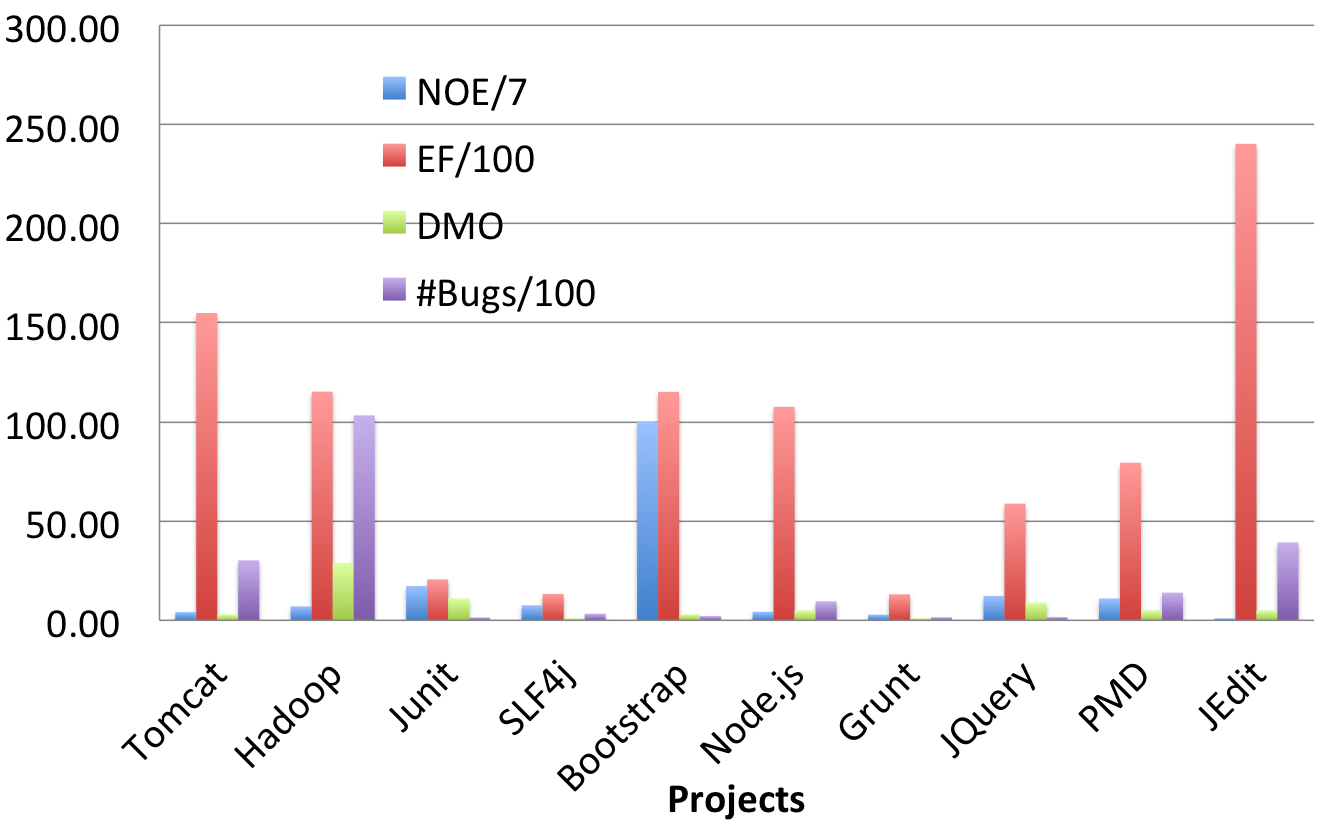
\includegraphics[scale=0.2]{figures/code-churn-metrics.png}
                    \caption{Repository Mining Tool Building}
                \end{figure}
        \end{frame}

    \subsection{Adoptability}
        \begin{frame}
            \frametitle{Adoptability}
            \textbf{Claim:}  Candoia apps are portable across diverse project settings and require no changes while adopting for new settings\\
            \textbf{Evaluation Strategy:}
            \begin{itemize}
                \item Implemted all 24 apps in Java for a project setting, keeping the tool modular and reusable
                \item Adopt the developed tool to new project setting
                \item Compared the LOC changes required in Candoia with Java to adopt a tool from a
                 project setting to another
            \end{itemize}
         \end{frame}

        \begin{frame}
            \frametitle{Project Settings Coverd by Test Projects}
            \begin{figure}[ht!] 
% \begin{footnotesize}
%\begin{scriptsize}
\centering
%\begin{minipage}{0.99\linewidth}
\begin{adjustbox}{max width=0.65\textwidth}
\begin{tabular}{|c|c|c|c|}
\hline
\rowcolor[HTML]{C0C0C0} 
\# & VCS & PL & Bugs \\
\hline\hline
1 & \inline{GIT} & \inline{Java} & \inline{Issues} \\ \hline
2 & \inline{SVN} & \inline{Java} & \inline{Bugzilla} \\ \hline
3 & \inline{GIT} & \inline{Java} & \inline{JIRA} \\ \hline
\end{tabular}
\end{adjustbox}
%\end{minipage}
%\begin{minipage}{0.99\linewidth}
\begin{adjustbox}{max width=0.65\textwidth}
\begin{tabular}{|c|c|c|c|}
\hline
\rowcolor[HTML]{C0C0C0} 
\# & VCS & PL & Bugs \\
\hline\hline
4 & \inline{GIT} & \inline{Java} & \inline{Tickets} \\ \hline
5 & \inline{SVN} & \inline{Java} & \inline{Tickets} \\ \hline
6 & \inline{GIT} & \inline{JS} & \inline{Issues} \\ \hline
\end{tabular}
\end{adjustbox}
%\end{minipage}
% \end{footnotesize}
%\end{scriptsize}
\caption{Six project settings}
\label{fig:project-settings}
\end{figure}
         \end{frame}

        \begin{frame}
            \frametitle{LOC changes in Boa v/s. Java}
            %\begin{figure*}
\begin{figure}
%\centering
%\resizebox{0.5\textwidth}{!}{%
\centering
\begin{adjustbox}{max width=\textwidth}
\begin{tabular}{|c|c|l|l|l|l|l|l|c|c|c|c|c|}
\hline
\rowcolor[HTML]{C0C0C0}
& \# & \multicolumn{6}{c}{Java} & \multicolumn{5}{c}{Candoia} \\ \hline
& & $M_{VCS}$ & $M_{Bug}$ & $M_{Forge}$ & $M_{Mining}$ & $M_{Visualize}$ &
\inline{Total} & \inline{Boa} & \inline{JS} & \inline{HTML} & \inline{CSS} &
\inline{Total} \\
\hline\hline

\multirow{6}{*}{\begin{sideways}Nullcheck\end{sideways}} 
& 1 & 125 & 157 & 20 & 143 & 53 & 498 & 59 & 12 & 34 & 0 & 105 \\ 
\cline{2-13} & 2 & 148 (-89,+112) & 117 (-119,+79) & 27 (-15,+22) & 156
(-43,+60) & 53 (-1,+1) & 501 (-267,+274) & 59 & 12 & 34 & 0 & 105 \\
\cline{2-13} & 3 & 125 (-2,+2) & 129 (-110,+82) & 20 (-1,+1) & 155 (-21,+33) &
53 (-1,+1) & 482 (-135,+118) & 59 & 12 & 34 & 0 & 105
\\
\cline{2-13} & 4 & 125 (-2,+2) & 115 (-111,+69) & 20 (-1,+1) & 167 (-18,+42) &
53 (-1,+1) & 480 (-133,+115) & 59 & 12 & 34 & 0 & 105
\\
\cline{2-13} & 5 & 148 (-89,+112) & 116 (-110,+69) & 27 (-15,+22) & 154
(-48,+59) & 53 (-1,+1) & 498 (-263,+263) & 59 & 12 & 34 & 0 & 105
\\
\cline{2-13} & 6 & 120 (-15,+10) & 157 (-1,+1) & 20 (-1,+1) & 147 (-13,+17) &
53 (-1,+1) & 497 (-31,+30) & 59 & 12 & 34 & 0 & 105
\\
\hline

\multirow{6}{*}{\begin{sideways}File Association\end{sideways}}
& 1 & 72 & 139 & 20 & 138 & 53 & 422 & 20 & 12 & 34 & 0 & 66 \\ 
\cline{2-13} & 2 & 125 (-38,+91) & 60 (-113,+34) & 27 (-15,+22) & 140 (-45,+47)
& 53 (-1,+1) & 405 (-212,+195) & 20 & 12 & 34 & 0 & 66 \\
\cline{2-13} & 3 & 72 (-1,+1) & 146 (-120,+127) & 20 (-1,+1) & 146 (-7,+15) & 53
(-1,+1) & 437 (-130,+145) & 20 & 12 & 34 & 0 & 66 \\ 
\cline{2-13} & 4 & 72 (-1,+1) & 115 (-106,+72) & 20 (-1,+1) & 137 (-4,+3) & 53
(-1,+1) & 397 (-113,+78) & 20 & 12 & 34 & 0 & 66 \\
\cline{2-13} & 5 & 125 (-38,+91) & 95 (-96,+52) & 27 (-15,+22) & 133 (-30,+25) &
53 (-1,+1) & 433 (-180,+191) & 20 & 12 & 34 & 0 & 66 \\
\cline{2-13} & 6 & 72 (-1,+1) & 139 (-1,+1) & 20 (-1,+1) & 138 (-1,+1) & 53
(-1,+1) & 421 (-5,+5) & 20 & 12 & 34 & 0 & 66 \\ \hline

\multirow{6}{*}{\begin{sideways}Churn Rate\end{sideways}}  
& 1 & 52 & 0 & 20 & 69 & 53 & 194 & 13 & 33 & 47 & 0 & 93 \\ 

\cline{2-13} & 2 & 104 (-38,+90) & 0 & 27 (-15,+22) & 74 (-26,+31) & 53 (-1,+1)
& 258 (-80,+144) & 13 & 33 & 47 & 0 & 93 \\

\cline{2-13} & 3 & 52 & 0 & 20 (-1,+1) & 69 & 53 (-1,+1) & 194 (-2,+2) & 13 & 33 & 47 & 0 & 93 \\ 

\cline{2-13} & 4 & 52 & 0 & 20 (-1,+1) & 69 & 53 (-1,+1) & 194 (-2,+2) & 13 & 33 & 47 & 0 & 93 \\

\cline{2-13} & 5 & 104 (-38,+90) & 0 & 27 (-15,+22) & 74 (-26,+31) & 53 (-1,+1)
& 258 (-80,+144) & 13 & 33 & 47 & 0 & 93 \\

\cline{2-13} & 6 & 52 & 0 & 20 (-1,+1) & 69 & 53 (-1,+1) & 194 (-2,+2)
& 13 & 33 & 47 & 0 & 93 \\ \hline

\multirow{6}{*}{\begin{sideways}BugSrc Mapper\end{sideways}}
& 1 & 78 & 152 & 20 & 73 & 53 & 376 & 37 & 30 & 47 & 32 & 146 \\ 

\cline{2-13} & 2 & 105 (-49,+76) & 79 (-118,+45) & 27 (-15,+22) & 74 (-41,+42) &
53 (-1,+1) & 338 (-224,+186) & 37 & 30 & 47 & 32 & 146 \\

\cline{2-13} & 3 & 78 (-2,+2) & 104 (-111,+63) & 20 (-1,+1) & 78 (-28,+33) & 53
(-1,+1) & 333 (-143,+100) & 37 & 30 & 47 & 32 & 146 \\

\cline{2-13} & 4 & 78 (-2,+2) & 85 (-106,+39) & 20 (-1,+1) & 77 (-24,+28) & 53
(-1,+1) & 313 (-134,+71) & 37 & 30 & 47 & 32 & 146 \\

\cline{2-13} & 5 & 108 (-44,+74) & 85 (-106,+39) & 27 (-15,+22) & 69 (-45,+41) &
53 (-1,+1) & 342 (-211,+177) & 37 & 30 & 47 & 32 & 146 \\

\cline{2-13} & 6 & 78 (-2,+2) & 152 (-1,+1) & 20 (-1,+1) & 78 (-28,+33) & 53
(-1,+1) & 381 (-33,+38) & 37 & 30 & 47 & 32 & 146 \\
\hline

% \multirow{6}{*}{\begin{sideways}Method Usage\end{sideways}}
% & 1 & a & b & c & d & e & f & p & q & r & s & t \\ \cline{2-13}
% & 2 & a & b & c & d & e & f & p & q & r & s & t \\ \cline{2-13}
% & 3 & a & b & c & d & e & f & p & q & r & s & t \\ \cline{2-13}
% & 4 & a & b & c & d & e & f & p & q & r & s & t \\ \cline{2-13}
% & 5 & a & b & c & d & e & f & p & q & r & s & t \\ \cline{2-13}
% & 6 & a & b & c & d & e & f & p & q & r & s & t \\ \hline
\end{tabular}
\end{adjustbox}
\caption{\tiny{Compares LOC changes required for adopting apps from one project
setting to another in Java and Candoia.}}
\label{fig:adoptability}
%}
%\end{figure*}
\end{figure}
         \end{frame}

        \begin{frame}
            \frametitle{LOC changes in Boa v/s. Java}
            %\begin{figure*}
\begin{figure}
%\centering
%\resizebox{0.5\textwidth}{!}{%
\centering
\begin{adjustbox}{max width=\textwidth}
\begin{tabular}{|c|c|l|l|l|l|l|l|c|c|c|c|c|}
\hline
\rowcolor[HTML]{C0C0C0}
& \# & \multicolumn{6}{c}{Java} & \multicolumn{5}{c}{Candoia} \\ \hline
& & $M_{VCS}$ & $M_{Bug}$ & $M_{Forge}$ & $M_{Mining}$ & $M_{Visualize}$ &
\inline{Total} & \inline{Boa} & \inline{JS} & \inline{HTML} & \inline{CSS} &
\inline{Total} \\
\hline\hline

    \multirow{6}{*}{\begin{sideways}File Association\end{sideways}}
    & 1 & 72 & 139 & 20 & 138 & 53 & 422 & 20 & 12 & 34 & 0 & 66 \\
    \cline{2-13} & 2 & 125 (-38,+91) & 60 (-113,+34) & 27 (-15,+22) & 140 (-45,+47)
    & 53 (-1,+1) & 405 (-212,+195) & 20 & 12 & 34 & 0 & 66 \\
    \cline{2-13} & 3 & 72 (-1,+1) & 146 (-120,+127) & 20 (-1,+1) & 146 (-7,+15) & 53
    (-1,+1) & 437 (-130,+145) & 20 & 12 & 34 & 0 & 66 \\
    \cline{2-13} & 4 & 72 (-1,+1) & 115 (-106,+72) & 20 (-1,+1) & 137 (-4,+3) & 53
    (-1,+1) & 397 (-113,+78) & 20 & 12 & 34 & 0 & 66 \\
    \cline{2-13} & 5 & 125 (-38,+91) & 95 (-96,+52) & 27 (-15,+22) & 133 (-30,+25) &
    53 (-1,+1) & 433 (-180,+191) & 20 & 12 & 34 & 0 & 66 \\
    \cline{2-13} & 6 & 72 (-1,+1) & 139 (-1,+1) & 20 (-1,+1) & 138 (-1,+1) & 53
    (-1,+1) & 421 (-5,+5) & 20 & 12 & 34 & 0 & 66 \\ \hline

\begin{comment}
\multirow{6}{*}{\begin{sideways}Churn Rate\end{sideways}}  
& 1 & 52 & 0 & 20 & 69 & 53 & 194 & 13 & 33 & 47 & 0 & 93 \\ 

\cline{2-13} & 2 & 104 (-38,+90) & 0 & 27 (-15,+22) & 74 (-26,+31) & 53 (-1,+1)
& 258 (-80,+144) & 13 & 33 & 47 & 0 & 93 \\

\cline{2-13} & 3 & 52 & 0 & 20 (-1,+1) & 69 & 53 (-1,+1) & 194 (-2,+2) & 13 & 33 & 47 & 0 & 93 \\ 

\cline{2-13} & 4 & 52 & 0 & 20 (-1,+1) & 69 & 53 (-1,+1) & 194 (-2,+2) & 13 & 33 & 47 & 0 & 93 \\

\cline{2-13} & 5 & 104 (-38,+90) & 0 & 27 (-15,+22) & 74 (-26,+31) & 53 (-1,+1)
& 258 (-80,+144) & 13 & 33 & 47 & 0 & 93 \\

\cline{2-13} & 6 & 52 & 0 & 20 (-1,+1) & 69 & 53 (-1,+1) & 194 (-2,+2)
& 13 & 33 & 47 & 0 & 93 \\ \hline
\end{comment}


\begin{comment}
\multirow{6}{*}{\begin{sideways}BugSrc Mapper\end{sideways}}
& 1 & 78 & 152 & 20 & 73 & 53 & 376 & 37 & 30 & 47 & 32 & 146 \\ 

\cline{2-13} & 2 & 105 (-49,+76) & 79 (-118,+45) & 27 (-15,+22) & 74 (-41,+42) &
53 (-1,+1) & 338 (-224,+186) & 37 & 30 & 47 & 32 & 146 \\

\cline{2-13} & 3 & 78 (-2,+2) & 104 (-111,+63) & 20 (-1,+1) & 78 (-28,+33) & 53
(-1,+1) & 333 (-143,+100) & 37 & 30 & 47 & 32 & 146 \\

\cline{2-13} & 4 & 78 (-2,+2) & 85 (-106,+39) & 20 (-1,+1) & 77 (-24,+28) & 53
(-1,+1) & 313 (-134,+71) & 37 & 30 & 47 & 32 & 146 \\

\cline{2-13} & 5 & 108 (-44,+74) & 85 (-106,+39) & 27 (-15,+22) & 69 (-45,+41) &
53 (-1,+1) & 342 (-211,+177) & 37 & 30 & 47 & 32 & 146 \\

\cline{2-13} & 6 & 78 (-2,+2) & 152 (-1,+1) & 20 (-1,+1) & 78 (-28,+33) & 53
(-1,+1) & 381 (-33,+38) & 37 & 30 & 47 & 32 & 146 \\
\hline

\end{comment}
% \multirow{6}{*}{\begin{sideways}Method Usage\end{sideways}}
% & 1 & a & b & c & d & e & f & p & q & r & s & t \\ \cline{2-13}
% & 2 & a & b & c & d & e & f & p & q & r & s & t \\ \cline{2-13}
% & 3 & a & b & c & d & e & f & p & q & r & s & t \\ \cline{2-13}
% & 4 & a & b & c & d & e & f & p & q & r & s & t \\ \cline{2-13}
% & 5 & a & b & c & d & e & f & p & q & r & s & t \\ \cline{2-13}
% & 6 & a & b & c & d & e & f & p & q & r & s & t \\ \hline
\end{tabular}
\end{adjustbox}
\caption{Compares LOC changes required for adopting apps from one project
setting to another in Java and Candoia.}
\label{fig:adoptability}
%}
%\end{figure*}
\end{figure}
         \end{frame}

 \subsection{Customizability}
        \begin{frame}
            \frametitle{Customizability}
            \textbf{Claim:} Performing customizations in Candoia requires less efforts in terms of LOC \\
            \textbf{Evaluation Criteria:}
            \begin{itemize}
                \item Customize the Java and Candoia apps
                \item Customizations include change in Mining logic, visualization, external tool usage etc.
                \item Compared the LOC changes required to customize the Candoia app with Java tool
            \end{itemize}
         \end{frame}

        \begin{frame}
%            \frametitle{LOC changes in Boa v/s. Java}
            \begin{figure}
\centering
\begin{scriptsize}
\begin{adjustbox}{max width=\textwidth}
\begin{tabular}{|c|c||c|c|}
\hline
$c_{10}$ & Shows number of nullcheck bug revisions in pie chart & $c_{23}$ &
Module association instead of file association \\
\hline 

$c_{11}$ & Change the output display to column chart & $c_{24}$ & File
association without bug data \\
\hline

$c_{12}$ & Display nullcheck issue life time & $c_{30}$ & Churn rate based on
revisions \\
\hline

$c_{13}$ & Plot nullcheck date v/s number of modified files & $c_{31}$ &
Associate bugs to churn rates \\
\hline 

$c_{14}$ & Maps nullcheck to developers & $c_{40}$ & Bugs to source files
mapping displayed in column chart \\
\hline

$c_{20}$ & File associations using weka apriori & $c_{41}$ & Change the output
display to pie chart \\
\hline

$c_{21}$ & File associations using weka fpgrowth & $c_{42}$ & Top five files
with maximum bug fix time \\
\hline

$c_{22}$ & File associations using spmf eclat & $c_{43}$ & Asssociate
developers to bugs \\
\hline
\end{tabular}
\end{adjustbox}
\end{scriptsize}

\begin{adjustbox}{max width=\textwidth}
\begin{tabular}{|c|c|l|l|l|l|l|l|l|l|l|l|l|}
\hline
\rowcolor[HTML]{C0C0C0}
& \# & \multicolumn{6}{c}{Java} & \multicolumn{5}{|c}{Candoia{}} \\ \hline
& & $M_{VCS}$ & $M_{Bug}$ & $M_{Forge}$ & $M_{Mining}$ & $
M_{Visualize}$ & \inline{Total} & \inline{Boa} & \inline{JS} & \inline{HTML} &
\inline{CSS} & \inline{Total} \\
\hline\hline

\multirow{5}{*}{\begin{sideways}Nullcheck\end{sideways}} 
& $c_{10}$ & 125 & 157 & 20 & 143 & 53 & 498 & 59 & 41 & 45 & 26 & 171 \\ 

\cline{2-13} & $c_{11}$ & 125 (-1,+1) & 157 (-1,+1) & 20 (-1,+1) & 143 (-2,+2) &
53 (-3,+3) & 498 (-8,+8) & 59 & 12 & 34 & 0 & 105
\\

\cline{2-13} & $c_{12}$ & 125 (-1,+1) & 137 (-29,+9) & 20 (-1,+1) & 144
(-14,+11) & 53 (-2,+2) & 479 (-47,+24) & 74 (-4,+19) & 41 (-2,+2) & 45 (-4,+4) &
26 (-1,+1) & 186 (-11,+26)
\\

\cline{2-13} & $c_{13}$ & 125 (-1,+1) & 157 (-1,+1) & 20 (-1,+1) & 147 (-6,+11)
& 53 (-1,+1) & 501 (-10,+15) & 64 (-3,+8) & 41 (-4,+4) & 45 (-4,+4) & 26 (-1,+1)
& 176 (-12,+17)
\\

\cline{2-13} & $c_{14}$ & 125 (-1,+1) & 157 (-1,+1) & 20 (-1,+1) & 147 (-13,+18)
& 53 (-1,+1) & 502 (-17,+22) & 61 (-4,+1) & 41 (-4,+4) & 45 (-4,+4) & 26 (-1,+1)
& 173 (-13,+10)
\\

\hline

\multirow{5}{*}{\begin{sideways}File Assoc.\end{sideways}} 
& $c_{20}$ & 141 & 157 & 20 & 178 & 23 & 481 & 37 & 12 & 34 & 0 & 83 \\
 
\cline{2-13} & $c_{21}$ & 141 (-1,+1) & 157 (-1,+1) & 20 (-1,+1) & 178 (-3,+3) &
23 (-1,+1) & 481 (-7,+7) & 37 & 12 (-1,+1) & 34 & 0 & 83 (-1,+1)
\\

\cline{2-13} & $c_{22}$ & 141 (-1,+1) & 157 (-1,+1) & 20 (-1,+1) & 183 (-23,+28)
& 23 (-1,+1) & 486 (-27,+32) & 37 & 12 (-1,+1) & 34 & 0 & 83 (-1,+1)
\\

\cline{2-13} & $c_{23}$ & 141 (-1,+1) & 157 (-1,+1) & 20 (-1,+1) & 178 (-3,+3) &
23 (-1,+1) & 461 (-8,+34) & 37 & 12 (-1,+1) & 34 & 0 & 83 (-1,+1)
\\

\cline{2-13} & $c_{24}$ & 141 (-1,+1) & 0 & 20 (-1,+1) & 175 (-5,+2) & 23
(-1,+1) & 359 (-165,+5) & 24 (-20,+7) & 12 (-1,+1) & 34 & 0 & 70 (-21,+8)
\\

\hline

\multirow{2}{*}{\begin{sideways}Churn\end{sideways}} 
& $c_{30}$ & 52 & 0 & 20 & 69 & 53 & 194 & 13 & 33 & 47 & 0 & 93 \\ 

\cline{2-13} & $c_{31}$ & 72 (-1,+21) & 0 & 20 (-1,+1) & 73 (-4,+8) & 53 (-1,+1)
& 218 (-7,+31) & 42 (-4,33) & 33 & 47 & 0 & 122 (-4,+33)
\\

\hline

\multirow{4}{*}{\begin{sideways}BugSrc\end{sideways}} 
& $c_{40}$ & 78 & 152 & 20 & 73 & 53 & 376 & 37 & 30 & 47 & 32 & 146 \\ 

\cline{2-13} & $c_{41}$ & 78 (-2,+2) & 152 (-2,+2) & 20 (-1,+1) & 73 (-1,+1) &
53 (-2,+2) & 376 (-8,+8) & 37 & 38 (-28,+35) & 47 & 32 & 154 (-28,+35)
\\

\cline{2-13} & $c_{42}$ & 78 (-2,+2) & 152 (-2,+2) & 20 (-1,+1) & 137 (-18,+82)
& 53 (-1,+1) & 440 (-24,+88) & 41 (-15,+19) & 30 & 47 & 32 & 155 (-15,+19)
\\
  
\cline{2-13} & $c_{43}$ & 78 (-2,+2) & 157 (-17,+23) & 20 (-1,+1) & 99 (-19,+47)
& 53 (-1,+1) & 407 (-40,+74) & 46 (-2,+11) & 38 (-4,+12) & 47 & 32 & 163
(-6,+23)
\\

\hline
\end{tabular}
\end{adjustbox}
\caption{\tiny{Compares LOC changes required for a number of customizations in Java and Candoia.}}
\label{fig:customizability}
\end{figure}
         \end{frame}

        \begin{frame}
%            \frametitle{LOC changes in Boa v/s. Java}
            \begin{figure}
\centering
\begin{scriptsize}
\begin{adjustbox}{max width=\textwidth}
\begin{tabular}{|c|c||c|c|}
\hline
$c_{10}$ & Shows number of nullcheck bug revisions in pie chart  \\
\hline 

$c_{11}$ & Change the output display to column chart  \\
\hline

$c_{12}$ & Display nullcheck issue life time\\
\hline

$c_{13}$ & Plot nullcheck date v/s number of modified files\\
\hline 

$c_{14}$ & Maps nullcheck to developers\\
\hline
\end{tabular}
\end{adjustbox}
\end{scriptsize}

\begin{adjustbox}{max width=\textwidth}
\begin{tabular}{|c|c|l|l|l|l|l|l|l|l|l|l|l|}
\hline
\rowcolor[HTML]{C0C0C0}
& \# & \multicolumn{6}{c}{Java} & \multicolumn{5}{|c}{Candoia{}} \\ \hline
& & $M_{VCS}$ & $M_{Bug}$ & $M_{Forge}$ & $M_{Mining}$ & $
M_{Visualize}$ & \inline{Total} & \inline{Boa} & \inline{JS} & \inline{HTML} &
\inline{CSS} & \inline{Total} \\
\hline\hline

\multirow{5}{*}{\begin{sideways}Nullcheck\end{sideways}}
& $c_{10}$ & 125 & 157 & 20 & 143 & 53 & 498 & 59 & 41 & 45 & 26 & 171 \\

\cline{2-13} & $c_{11}$ & 125 (-1,+1) & 157 (-1,+1) & 20 (-1,+1) & 143 (-2,+2) &
53 (-3,+3) & 498 (-8,+8) & 59 & 12 & 34 & 0 & 105
\\

\cline{2-13} & $c_{12}$ & 125 (-1,+1) & 137 (-29,+9) & 20 (-1,+1) & 144
(-14,+11) & 53 (-2,+2) & 479 (-47,+24) & 74 (-4,+19) & 41 (-2,+2) & 45 (-4,+4) &
26 (-1,+1) & 186 (-11,+26)
\\

\cline{2-13} & $c_{13}$ & 125 (-1,+1) & 157 (-1,+1) & 20 (-1,+1) & 147 (-6,+11)
& 53 (-1,+1) & 501 (-10,+15) & 64 (-3,+8) & 41 (-4,+4) & 45 (-4,+4) & 26 (-1,+1)
& 176 (-12,+17)
\\

\cline{2-13} & $c_{14}$ & 125 (-1,+1) & 157 (-1,+1) & 20 (-1,+1) & 147 (-13,+18)
& 53 (-1,+1) & 502 (-17,+22) & 61 (-4,+1) & 41 (-4,+4) & 45 (-4,+4) & 26 (-1,+1)
& 173 (-13,+10)
\\

\hline

\hline
\end{tabular}
\end{adjustbox}
\caption{Compares LOC changes required for a number of customizations in Java and Candoia.}
\label{fig:customizability}
\end{figure}
         \end{frame}
  \section*{Related Work}
\subsection{Related Work}
    \begin{frame}
       \begin{columns}
            \column{0.5\textwidth}
                Platforms for reusing of tools
                \begin{itemize}
                    \item Moose
                    \item RepoGrams
                    \item Kenyon and Sourcerer
                    \item Alitheia Core
                    \item FLOSSMole
                    \item Groundhog
                \end{itemize}

            \column{0.5\textwidth}
                Provides a repository of datasets
                \begin{itemize}
                    \item GHTorrent
                    \item Promise Repository
                    \item SourcererDB
                    \item Boa
                \end{itemize}
        \end{columns}
    \end{frame}

\section{Summary}
    \subsection{Summary}
        \begin{frame}
            \begin{figure}
                \centering
                    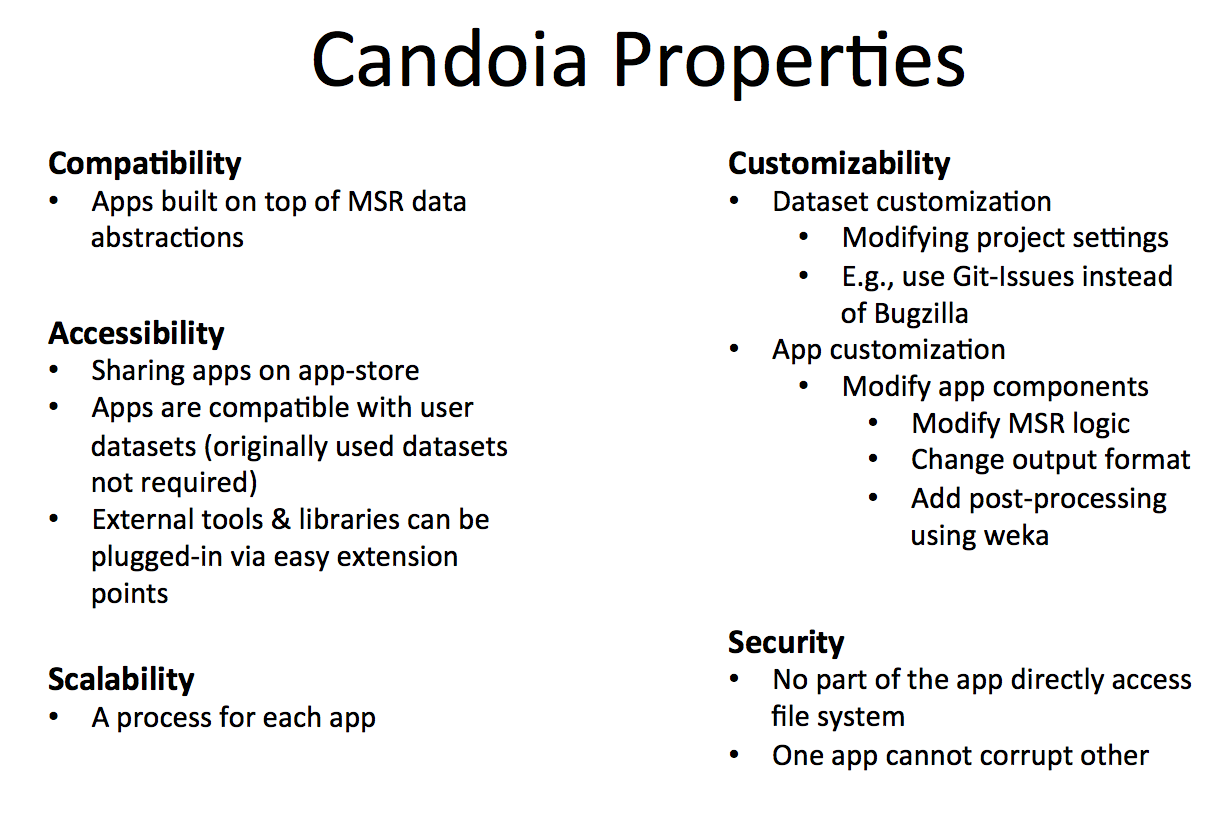
\includegraphics[scale=0.2]{figures/summary.png}
            \end{figure}
        \end{frame}


\makeatletter % to change template
    \setbeamertemplate{headline}[default] % not mandatory, but I though it was better to set it blank
    \def\beamer@entrycode{\vspace*{-\headheight}} % here is the part we are interested in :)
\makeatother

        \begin{frame}
                \begin{figure}
                    \centering
                    
\includegraphics[scale=0.2]{figures/thankyou.png}
                \end{figure}
        \end{frame}




  \appendix

% make sure you have a blank slide in case you accidentally go past your conclusion
\begin{frame}[plain]
\end{frame}


% these slides are to help answer potential questions and generally arent shown
% unless needed or there is extra time
\begin{frame}[plain]{Logistic Regression}
Logistic regression,
\begin{figure}
\centering
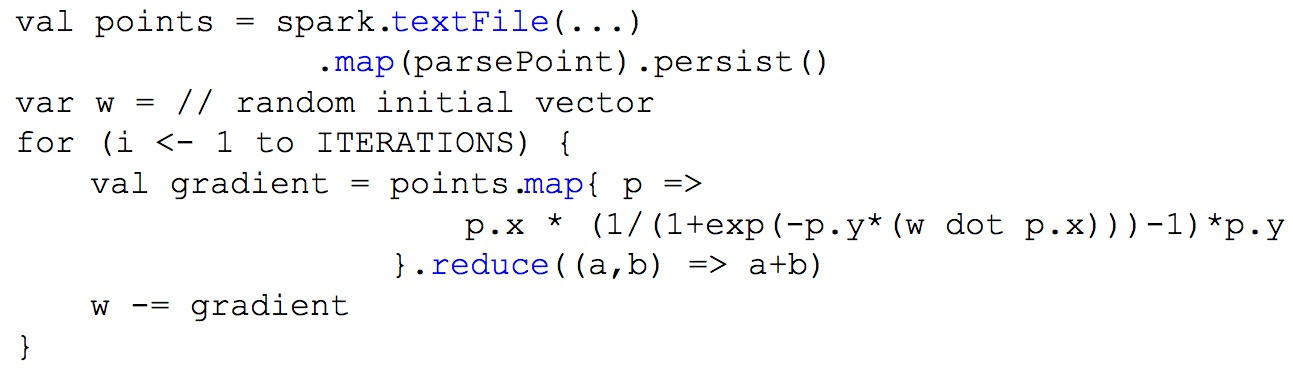
\includegraphics[width=0.9\linewidth]{figures/logistic-regression.jpg}
\end{figure}
\begin{itemize}
  \item \texttt{points} is a persistent RDD produced by \texttt{map} on text
  file
  \item repeatedly run \texttt{map} and \texttt{reduce} to compute gradient at
  each step by summing function of the current w.
  \item keeping \texttt{points} in memory across iterations yields 20x speedup.
\end{itemize}
\end{frame}

\begin{frame}[plain]{Word Count}
\begin{figure}
\centering
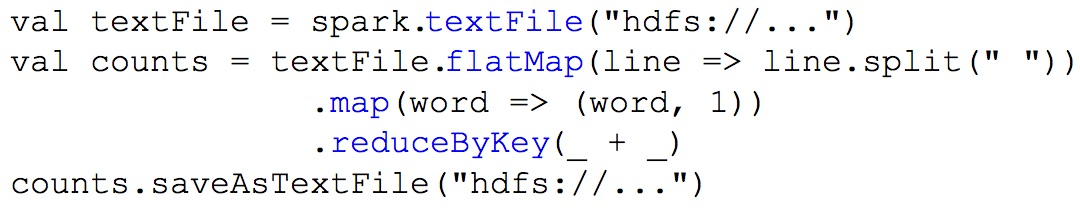
\includegraphics[width=0.9\linewidth]{figures/word-count.jpg}
\end{figure}
\end{frame}

\begin{frame}[plain]{Performance Tuning}
Problems,
\begin{itemize}
  \item Too few partitions
  \item Large per-key \texttt{groupBy()}
  \item Shipped all data across the cluster 
\end{itemize}

Guidelines
\begin{itemize}
  \item Ensure enough partitions (often 100 - 10000), mostly based on task
  execution time at least 100ms (upper bound), at least ~2x number of cores in
  cluster (lower bound)
  \item Minimize memory consumption while sorting and large keys in groupBys
  \item Minimize amount of data shuffled  
\end{itemize}

Resolution
\begin{itemize}
  \item Increase \texttt{spark.executor.memory}
  \item Increase number of partitions
  \item Re-evaluate program structure   
\end{itemize}
\end{frame}

\begin{frame}[plain]{Example 2 Optimization}
\begin{figure}
\centering
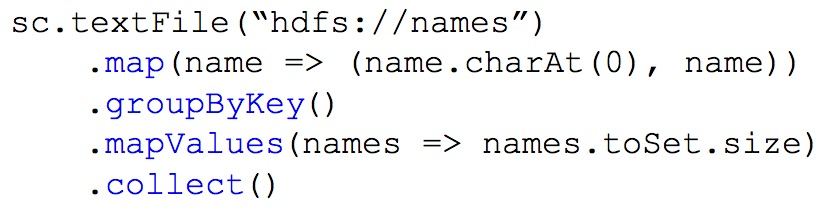
\includegraphics[width=0.9\linewidth]{figures/example2.jpg}
\end{figure}

\begin{figure}
\centering

\includegraphics[width=0.9\linewidth]{figures/example2-optimized.jpg}
\end{figure}
\end{frame}


\end{document}
